\documentclass[11pt,a4paper]{article}
\usepackage[T1]{fontenc}
\usepackage[utf8]{inputenc}
\usepackage{mathpazo}
\usepackage[scaled=0.92]{helvet}
\usepackage{babel}
\babelprovide[import, main]{portuguese}
\usepackage[margin=2cm,top=2.3cm,bottom=2.2cm]{geometry}
\usepackage{amsmath,amssymb,mathtools}
\usepackage{xcolor}
\usepackage{tikz}
\usetikzlibrary{arrows.meta,calc,decorations.pathreplacing,patterns}
\usepackage[most]{tcolorbox}
\usepackage{booktabs,array,multicol,enumitem,fancyhdr,microtype}
\usepackage{cancel}
\usepackage[hidelinks]{hyperref}

\emergencystretch=1.5em
\tolerance=1500
\setlength{\parindent}{0pt}
\setlength{\parskip}{4pt plus 1pt}

% ---------- cores ----------
\definecolor{azul}{HTML}{1F4E79}
\definecolor{azulclaro}{HTML}{EAF1F8}
\definecolor{verde}{HTML}{1B6E4A}
\definecolor{verdeclaro}{HTML}{E8F4EE}
\definecolor{vermelho}{HTML}{A3282C}
\definecolor{vermelhoclaro}{HTML}{FBECEC}
\definecolor{roxo}{HTML}{5B3C88}
\definecolor{roxoclaro}{HTML}{F0EBF7}
\definecolor{cinza}{HTML}{555555}
\definecolor{cinzaclaro}{HTML}{F3F3F3}
\definecolor{laranja}{HTML}{B5651D}
\definecolor{laranjaclaro}{HTML}{FCF1E6}
\definecolor{amarelo}{HTML}{8A6D00}
\definecolor{amareloclaro}{HTML}{FFF8DC}

% cores dos símbolos da soma de Riemann (usadas na "anatomia")
\definecolor{cLim}{HTML}{5B3C88}
\definecolor{cSum}{HTML}{B5651D}
\definecolor{cF}{HTML}{1B6E4A}
\definecolor{cX}{HTML}{A3282C}
\definecolor{cDx}{HTML}{1F4E79}

% ---------- macros ----------
\DeclareMathOperator{\sen}{sen}
\DeclareMathOperator{\tg}{tg}
\DeclareMathOperator{\cotg}{cotg}
\DeclareMathOperator{\cossec}{cossec}
\DeclareMathOperator{\arctg}{arctg}
\DeclareMathOperator{\arcsen}{arcsen}
\DeclareMathOperator{\senh}{senh}
\newcommand{\dx}{\,dx}
\newcommand{\dt}{\,dt}
\newcommand{\du}{\,du}
\newcommand{\R}{\mathbb{R}}
\newcommand{\ok}{\textcolor{verde}{\checkmark}}
\usepackage{pifont}\newcommand{\bad}{\textcolor{vermelho}{\ding{55}}}
\newcommand{\eval}[2]{\Big|_{#1}^{#2}}

% ---------- caixas ----------
\tcbset{
  base/.style={enhanced, breakable, boxrule=0.6pt, arc=2pt, left=6pt, right=6pt, top=4pt, bottom=4pt,
               fonttitle=\bfseries\sffamily, before skip=6pt, after skip=8pt},
}
\newtcolorbox{definicao}[1][]{base, colback=azulclaro, colframe=azul, title={#1}}
\newtcolorbox{metodo}[1][]{base, colback=verdeclaro, colframe=verde, title={#1}}
\newtcolorbox{armadilha}[1][Armadilha de prova]{base, colback=vermelhoclaro, colframe=vermelho, title={#1}}
\newtcolorbox{geo}[1][Interpretação geométrica]{base, colback=roxoclaro, colframe=roxo, title={#1}}
\newtcolorbox{exemplo}[1][]{base, colback=cinzaclaro, colframe=cinza, title={#1}}
\newtcolorbox{exercicios}[1][Exercícios similares]{base, colback=amareloclaro, colframe=amarelo, title={#1}}
\newtcolorbox{dica}[1][Na prova]{base, colback=laranjaclaro, colframe=laranja, title={#1}}

% ---------- cabeçalho ----------
\pagestyle{fancy}
\fancyhf{}
\fancyhead[L]{\sffamily\small Cálculo II --- Resumo para a Prova 1}
\fancyhead[R]{\sffamily\small\nouppercase{\leftmark}}
\fancyfoot[C]{\sffamily\small\thepage}
\renewcommand{\headrulewidth}{0.4pt}

\setcounter{secnumdepth}{2}
\setcounter{tocdepth}{1}

\begin{document}
\thispagestyle{empty}
\begin{center}
\vspace*{1.2cm}
{\sffamily\bfseries\Huge Cálculo II}\\[6pt]
{\sffamily\bfseries\LARGE Resumo para a Prova 1}\\[18pt]
{\sffamily\large Somas de Riemann \;\textperiodcentered\; Integrais definidas e indefinidas \;\textperiodcentered\; Como \emph{ler} uma derivada}\\[8pt]
{\small Baseado nas questões recomendadas pela professora --- Stewart, \emph{Cálculo}, vol.~1, 9\textsuperscript{a} ed., seções 4.9 a 6.3}\\[4pt]
{\small Ciência da Computação --- 2\textsuperscript{o} período --- PUC Minas --- \today}
\end{center}

\vspace{0.6cm}

\begin{tcolorbox}[base, colback=azulclaro, colframe=azul, title={Como usar este resumo}]
\begin{itemize}[leftmargin=1.4em, itemsep=2pt]
\item \textbf{Parte 1} é a base: se você lê corretamente o que uma derivada \emph{significa}, toda integral vira ``desfazer uma derivada'' e todo teorema do capítulo 5 vira óbvio.
\item \textbf{Parte 3} (somas de Riemann) é o coração da prova: cada símbolo da fórmula é explicado, com um exemplo completo calculado de três formas diferentes (soma com $n=6$, limite exato, TFC) --- e as três batem.
\item Cada exemplo resolvido segue o padrão: \emph{classificar} $\to$ \emph{resolver sem pular passos} $\to$ \emph{interpretar geometricamente} $\to$ \emph{verificar}. Depois de cada seção há exercícios similares; o gabarito está no fim.
\item As caixas \textcolor{vermelho}{\textbf{vermelhas}} são os erros que custam ponto. Leia-as duas vezes.
\end{itemize}
\end{tcolorbox}

\tableofcontents
\newpage

\section{Escopo da Prova 1 e o que cada seção cobra}

A lista da professora (tabela de questões) vai de 4.9 até 6.3 antes de mudar de formato (7.1 em diante é ``aquecimento / lista completa'', material da P2). O cronograma das aulas 02--05 detalha as primeiras seções. Cruzando os dois:

\begin{center}
\small
\renewcommand{\arraystretch}{1.25}
\begin{tabular}{@{}p{1.0cm}>{\raggedright\arraybackslash}p{2.9cm}>{\raggedright\arraybackslash}p{3.4cm}>{\raggedright\arraybackslash}p{8.3cm}@{}}
\toprule
\textbf{Seção} & \textbf{Tema} & \textbf{Questões recomendadas} & \textbf{Tipo de questão que isso gera na prova}\\
\midrule
4.9 & Primitivas & 1--26; 29--54; 55; 56; 65--70 & primitiva mais geral; achar $f$ a partir de $f'$ ou $f''$ com condições; reta tangente dada; cinemática $a\to v\to s$\\
5.1 & Áreas e distâncias & 2, 3, 11, 20, 24 (aula 04); 16--23 & estimar área com $L_n$, $R_n$, $M_n$ e dizer se é sub/superestimativa; escrever a área como limite; reconhecer a região dada por um limite\\
5.2 & Integral definida & 1, 3, 19--22, 23, 25--34, 41--46, 49, 50 & calcular soma de Riemann com $n$ dado \emph{e dizer o que ela representa}; limite $\leftrightarrow$ integral; calcular pela definição (Teorema 4); calcular por áreas\\
5.3 & TFC & 9, 10, 21--24, 25--54, 85, 86 & derivar $\int_a^{x} f(t)\dt$ (com regra da cadeia); calcular pelo TFC2 e interpretar como área; reconhecer um limite como soma de Riemann em $[0,1]$\\
5.4 & Integral indefinida e Variação Total & 1--24; 27--54; 57; 59--62; 69--74 & verificar fórmula por derivação; integral indefinida geral; definidas; interpretar $\int$ taxa; deslocamento $\times$ distância; massa, vazão\\
5.5 & Substituição & 1--8; 9--54; 59--80; 86--88 & substituição $u$ em indefinidas e definidas (trocando limites); simetria par/ímpar\\
6.1 & Área entre curvas & 1--6; 11--25 & esboçar, achar interseções, integrar em $x$ ou em $y$\\
6.2 & Volumes & 1--40 & discos e anéis; eixos deslocados ($y=k$, $x=k$)\\
6.3 & Cascas cilíndricas & 2--6; 9; 10; 25--30 & cascas; escolher entre cascas e anéis\\
\bottomrule
\end{tabular}
\end{center}

\begin{dica}[{O que \emph{não} cai na P1 --- e o que isso muda}]
Integração por partes, frações parciais e substituição trigonométrica são do capítulo 7 (P2). Portanto, na P1 a ``classificação da técnica'' se reduz a quatro opções:
\begin{enumerate}[leftmargin=1.6em, itemsep=1pt]
\item \textbf{Tabela direta} após preparação algébrica (expandir, dividir termo a termo, identidade trigonométrica) --- seções 4.9, 5.3, 5.4;
\item \textbf{Substituição $u$} quando há função composta acompanhada da derivada ``de dentro'' --- seção 5.5;
\item \textbf{Interpretação geométrica} (retângulo, triângulo, trapézio, semicírculo, valor absoluto) --- seção 5.2;
\item \textbf{Definição} como limite de somas de Riemann, quando o enunciado manda --- seções 5.1, 5.2.
\end{enumerate}
Se você se pegar tentando ``por partes'' na P1, pare: a questão está pedindo uma das quatro acima.
\end{dica}

\section{Derivadas: interpretar, não decorar}

Tudo no capítulo 5 é construído sobre uma única frase: \emph{integrar é desfazer uma derivada}. Se a derivada é só uma tabela decorada, a integral vira uma segunda tabela decorada --- e as questões conceituais (V/F, ``o que representa'', ``interprete'') ficam impossíveis. Esta parte fixa as leituras que você vai usar em todas as outras.

\subsection{As três leituras de $f'(a)$}

\begin{definicao}[{Definição}]
\[
f'(a)\;=\;\lim_{h\to 0}\frac{f(a+h)-f(a)}{h}
\]
O quociente é uma \emph{taxa média} (variação de $f$ dividida pela variação de $x$). O limite torna a taxa \emph{instantânea}.
\end{definicao}

\begin{enumerate}[leftmargin=1.6em, itemsep=3pt]
\item \textbf{Taxa de variação.} $f'(a)$ é ``quanto $f$ varia por unidade de $x$'' quando $x = a$. Unidade: $\dfrac{[\,f\,]}{[\,x\,]}$. Se $s$ é posição em metros e $t$ em segundos, $s'(t)$ está em m/s.
\item \textbf{Inclinação.} $f'(a)$ é o coeficiente angular da reta tangente ao gráfico em $(a, f(a))$:
$\;y = f(a) + f'(a)(x-a)$.
\item \textbf{Fator de aproximação linear} --- a leitura que mais importa para integrais:
\[
f(a+h)\approx f(a) + f'(a)\,h \qquad\Longleftrightarrow\qquad \Delta f \approx f'(a)\,\Delta x .
\]
Em palavras: num pedaço pequeno $\Delta x$, a função varia aproximadamente \emph{taxa} $\times$ \emph{largura do pedaço}. Uma soma de Riemann (Parte 3) é exatamente a soma desses pedaços: $\sum f'(x_i^*)\,\Delta x$ acumula a variação total. O Teorema da Variação Total (Parte 4) diz que, no limite, isso é exato: $\int_a^b f'(x)\dx = f(b)-f(a)$.
\end{enumerate}

\begin{definicao}[{Dicionário de derivadas em enunciados (aparece em 5.4 e nas questões de interpretação)}]
\small
\begin{tabular}{@{}>{\raggedright\arraybackslash}p{4.9cm}>{\raggedright\arraybackslash}p{7.3cm}>{\raggedright\arraybackslash}p{3.1cm}@{}}
\toprule
\textbf{Função} & \textbf{Derivada} & \textbf{Unidade da derivada}\\
\midrule
$s(t)$ posição (m) & $s'(t)=v(t)$ velocidade; $v'(t)=a(t)$ aceleração & m/s; m/s$^2$\\
$C(x)$ custo de produzir $x$ unidades (R\$) & $C'(x)$ custo marginal $\approx$ custo da próxima unidade & R\$/unidade\\
$m(x)$ massa da barra até o ponto $x$ (kg) & $m'(x)=\rho(x)$ densidade linear & kg/m\\
$V(t)$ volume no tanque (L) & $V'(t)$ vazão líquida (entra $-$ sai) & L/min\\
$Q(t)$ carga (C) & $Q'(t)=I(t)$ corrente & A $=$ C/s\\
$n(t)$ população & $n'(t)$ taxa de crescimento & indivíduos/semana\\
$w(t)$ peso de uma criança (kg) & $w'(t)$ taxa de crescimento & kg/ano\\
\bottomrule
\end{tabular}

\smallskip
Regra: a derivada de ``quantidade acumulada'' é ``taxa''. A integral faz o caminho de volta: a integral da taxa é a variação da quantidade acumulada (Parte 4).
\end{definicao}

\subsection{O que o sinal e o gráfico de $f'$ dizem sobre $f$}

\begin{itemize}[leftmargin=1.4em, itemsep=2pt]
\item $f'>0$ em um intervalo $\Rightarrow$ $f$ crescente ali; $f'<0$ $\Rightarrow$ decrescente. (O sinal de $f'$ fala da \emph{monotonia} de $f$, não do sinal de $f$.)
\item $f'(c)=0$ ou $f'(c)$ não existe $\Rightarrow$ $c$ é ponto crítico: \emph{candidato} a extremo, sem garantia ($f(x)=x^3$ em $c=0$).
\item $f''>0$ $\Rightarrow$ concavidade para cima ($f'$ crescente); $f''<0$ $\Rightarrow$ para baixo.
\item Derivável em $a$ $\Rightarrow$ contínua em $a$ $\Rightarrow$ $f(a)$ existe, ou seja, $a\in \mathrm{Dom}\,f$. A recíproca falha: $|x|$ é contínua em $0$ e não é derivável em $0$.
\end{itemize}

\begin{armadilha}[{Verdadeiro ou falso --- o estilo de questão conceitual da professora}]
\begin{itemize}[leftmargin=1.4em, itemsep=2pt]
\item ``Se $f'$ é crescente, então $f$ é crescente.'' \textbf{Falso.} $f'$ crescente é concavidade para cima. $f(x)=x^2$: $f'(x)=2x$ é crescente, mas $f$ decresce em $x<0$.
\item ``Se $f$ é decrescente, então $f'$ é decrescente.'' \textbf{Falso.} $f(x)=1/x$ em $(0,\infty)$ decresce, mas $f'(x)=-1/x^2$ \emph{cresce}.
\item ``Se $f'(a)=g'(a)$, então $f(a)=g(a)$.'' \textbf{Falso.} $f(x)=x^2$ e $g(x)=x^2+5$ têm a mesma derivada em todo ponto.
\item ``Se $F'=G'$ em um \emph{intervalo}, então $F-G$ é constante.'' \textbf{Verdadeiro} --- é o teorema das primitivas (Parte 2). Sem a palavra \emph{intervalo}, é falso.
\item ``Se $f$ é derivável em $a$, então é contínua em $a$.'' \textbf{Verdadeiro.} ``Se é contínua em $a$, então é derivável em $a$.'' \textbf{Falso} ($|x|$).
\item ``Se $f$ é contínua em $a$, então $a$ pertence ao domínio de $f$.'' \textbf{Verdadeiro}: continuidade exige que $f(a)$ exista.
\item ``Se $f'(c)=0$, então $f$ tem máximo ou mínimo em $c$.'' \textbf{Falso} ($x^3$ em $0$).
\end{itemize}
Método para V/F: tente um contraexemplo simples ($x^2$, $x^3$, $1/x$, $|x|$, uma constante somada). Se nenhum funciona, procure o teorema que garante a afirmação.
\end{armadilha}

\subsection{A tabela de derivadas lida ao contrário \emph{é} a tabela de integrais}

\begin{definicao}[{Uma tabela só, lida nos dois sentidos}]
\[
\frac{d}{dx}\big[F(x)\big] = f(x)
\qquad\Longleftrightarrow\qquad
\int f(x)\dx = F(x) + C
\]
\small
\renewcommand{\arraystretch}{1.55}
\begin{tabular}{@{}lcl@{\qquad}lcl@{}}
\toprule
$F(x)$ & $\xrightarrow{\;d/dx\;}$ & $f(x)$ & $F(x)$ & $\xrightarrow{\;d/dx\;}$ & $f(x)$\\
\midrule
$\dfrac{x^{n+1}}{n+1}$ ($n\neq -1$) & & $x^n$ & $\tg x$ & & $\sec^2 x$\\[6pt]
$\ln|x|$ & & $\dfrac1x$ & $-\cotg x$ & & $\cossec^2 x$\\[6pt]
$e^x$ & & $e^x$ & $\sec x$ & & $\sec x\,\tg x$\\[4pt]
$\dfrac{a^x}{\ln a}$ & & $a^x$ & $-\cossec x$ & & $\cossec x\,\cotg x$\\[6pt]
$\sen x$ & & $\cos x$ & $\arctg x$ & & $\dfrac{1}{1+x^2}$\\[6pt]
$-\cos x$ & & $\sen x$ & $\arcsen x$ & & $\dfrac{1}{\sqrt{1-x^2}}$\\[6pt]
$\senh x$ & & $\cosh x$ & $\cosh x$ & & $\senh x$\\
\bottomrule
\end{tabular}

\smallskip
Cada linha da coluna ``integrais'' não é um fato novo: é uma derivada que você já sabe, lida da direita para a esquerda. Consequência prática: \textbf{toda integral pode ser conferida derivando o resultado} --- faça isso na prova, leva 10 segundos.
\end{definicao}

Dois pontos onde ``decorar'' falha e ``ler'' salva:

\begin{itemize}[leftmargin=1.4em, itemsep=2pt]
\item \textbf{Por que $\int \sen x\dx = -\cos x + C$?} Porque $(-\cos x)' = -(-\sen x) = \sen x$. O sinal de menos vem da derivada do cosseno, não de uma convenção. Se você lembrar que $(\cos x)'=-\sen x$, nunca erra o sinal.
\item \textbf{Por que $x^{-1}$ é a exceção da regra da potência?} A fórmula $\frac{x^{n+1}}{n+1}$ dividiria por zero. A primitiva é $\ln|x|$ porque $(\ln|x|)' = 1/x$ para todo $x\neq 0$.
\end{itemize}

\subsection{Regra da cadeia lida ao contrário (ponte para a substituição)}

\[
\frac{d}{dx}\Big[F\big(g(x)\big)\Big] = F'\big(g(x)\big)\,g'(x) = f\big(g(x)\big)\,g'(x)
\qquad\Longrightarrow\qquad
\int f\big(g(x)\big)\,g'(x)\dx = F\big(g(x)\big)+C .
\]
Exemplo: $\dfrac{d}{dx}\sen(x^4+2) = \cos(x^4+2)\cdot 4x^3$; logo $\displaystyle\int x^3\cos(x^4+2)\dx = \tfrac14\sen(x^4+2)+C$. A Parte 5 é só isto, sistematizado.

\subsection{Derivada de integral, integral de derivada --- três expressões que parecem iguais}

\begin{exemplo}[{Exemplo 1.1 --- questão 8 da revisão do capítulo 5, adaptada}]
Compare:
\[
\text{(a) } \int_0^1 \frac{d}{dx}\Big[e^{\arctg x}\Big]\dx
\qquad
\text{(b) } \frac{d}{dx}\int_0^1 e^{\arctg x}\dx
\qquad
\text{(c) } \frac{d}{dx}\int_0^x e^{\arctg t}\dt
\]
\textbf{(a)} Integral de uma derivada em $[0,1]$ = variação líquida (TFC2): $e^{\arctg 1}-e^{\arctg 0} = e^{\pi/4}-e^{0} = e^{\pi/4}-1$. É um \emph{número}.

\textbf{(b)} $\int_0^1 e^{\arctg x}\dx$ tem limites constantes: é um número (uma área). Derivada de constante: \textbf{0}.

\textbf{(c)} O limite superior é a variável $x$: a integral é uma \emph{função} de $x$ (``área até $x$''), e o TFC1 dá $e^{\arctg x}$.

\medskip
Regra de leitura: \textbf{olhe os limites}. Constantes $\to$ número (derivada 0). Variável em cima $\to$ função, e derivar devolve o integrando. Derivada \emph{dentro} da integral $\to$ variação líquida $F(b)-F(a)$.
\end{exemplo}

\begin{exercicios}[{Exercícios similares --- Parte 1}]
\begin{enumerate}[leftmargin=1.6em, itemsep=2pt, label=\textbf{1.\arabic*}]
\item Verdadeiro ou falso, com justificativa: (a) se $f'(x)>0$ para todo $x$, então $f(x)>0$ para todo $x$; (b) se $f$ e $g$ são deriváveis e $f(x)-g(x)=3$ para todo $x$, então $f'=g'$; (c) se $f$ não é derivável em $a$, então $f$ não é contínua em $a$.
\item Se $V(t)$ é o volume de água (litros) em um tanque no instante $t$ (min), o que significa $V'(3)=-12$? Qual a unidade?
\item Calcule (a) $\displaystyle\int_0^{\pi}\frac{d}{dx}\big[x\sen x\big]\dx$; \;(b) $\displaystyle\frac{d}{dx}\int_0^{\pi} x\sen x\dx$; \;(c) $\displaystyle\frac{d}{dx}\int_0^{x} t\sen t\dt$.
\item Sem calcular a integral, diga se $\displaystyle\int_1^2 \ln x\dx$ é positivo ou negativo e por quê.
\end{enumerate}
\end{exercicios}

\section{Primitivas e integrais indefinidas (4.9 e 5.4)}

\subsection{Definição e o teorema da constante}

\begin{definicao}[{Primitiva}]
$F$ é uma \textbf{primitiva} de $f$ em um intervalo $I$ se $F'(x)=f(x)$ para todo $x\in I$.

\textbf{Teorema.} Se $F$ é uma primitiva de $f$ em um \emph{intervalo} $I$, então a primitiva mais geral de $f$ em $I$ é
\[
F(x)+C,\qquad C\in\R .
\]
\emph{Por quê:} se $G$ também é primitiva, então $(G-F)'=G'-F'=f-f=0$ em $I$; uma função com derivada zero em um intervalo é constante (corolário do Teorema do Valor Médio). Logo $G=F+C$.
\end{definicao}

\begin{armadilha}[{A palavra ``intervalo'' não é enfeite}]
Para $f(x)=1/x$, o domínio $(-\infty,0)\cup(0,\infty)$ \emph{não} é um intervalo. A primitiva mais geral é
\[
F(x)=\begin{cases}\ln|x|+C_1, & x>0\\ \ln|x|+C_2, & x<0\end{cases}
\]
com constantes que podem ser \emph{diferentes} em cada ramo. Escrever ``$\ln|x|+C$'' é a abreviação usual, válida em cada intervalo separadamente. Questão V/F típica: ``se $F'=G'$ então $F-G$ é constante'' --- só é verdadeiro em um intervalo.
\end{armadilha}

\begin{geo}
A família $F(x)+C$ é um feixe de curvas obtidas por translação vertical: todas têm, em cada $x$, retas tangentes \emph{paralelas} (mesma inclinação $f(x)$). Uma condição inicial ($F(x_0)=y_0$) escolhe \emph{uma} curva do feixe; por isso ``achar $f$ dado $f'$ e $f(0)$'' tem resposta única, e ``achar $f$ dado $f''$'' precisa de \emph{duas} condições (duas constantes).
\end{geo}

\subsection{Notação: integral indefinida $\neq$ integral definida}

\[
\int f(x)\dx = F(x)+C \quad\text{significa}\quad F'(x)=f(x).
\]
\begin{itemize}[leftmargin=1.4em, itemsep=2pt]
\item $\displaystyle\int f(x)\dx$ é uma \textbf{família de funções} (uma para cada $C$).
\item $\displaystyle\int_a^b f(x)\dx$ é um \textbf{número} (limite de somas de Riemann, Parte 3).
\item A ponte entre os dois é o TFC2 (Parte 4): $\displaystyle\int_a^b f(x)\dx = \Big[\int f(x)\dx\Big]_a^b = F(b)-F(a)$ --- e o $C$ cancela.
\end{itemize}

\subsection{Método: cinco passos para qualquer integral da P1}

\begin{metodo}[{Procedimento}]
\begin{enumerate}[leftmargin=1.6em, itemsep=2pt]
\item \textbf{Classificar.} Está na tabela direto? Precisa de preparação algébrica? Há função composta acompanhada da derivada ``de dentro'' (substituição, Parte 5)?
\item \textbf{Preparar.} Expandir produtos; dividir o numerador termo a termo pelo denominador; raízes $\to$ expoentes fracionários; $1/x^k\to x^{-k}$; identidades trigonométricas.
\item \textbf{Integrar termo a termo} (linearidade: $\int (cf+g) = c\int f + \int g$), usando a tabela.
\item \textbf{$+\,C$} (indefinida) ou \textbf{avaliar} $F(b)-F(a)$ (definida).
\item \textbf{Verificar derivando.} O resultado derivado tem que dar o integrando original.
\end{enumerate}
\end{metodo}

\begin{definicao}[{Catálogo de preparação algébrica --- o que mais aparece em 4.9/5.3/5.4}]
\small
\begin{tabular}{@{}ll@{\qquad}ll@{}}
\toprule
\textbf{Está assim} & \textbf{Reescreva} & \textbf{Está assim} & \textbf{Reescreva}\\
\midrule
$(x+1)(x-3)$ & $x^2-2x-3$ & $\tg^2 x$ & $\sec^2 x - 1$\\[2pt]
$\dfrac{2+x^2}{\sqrt{x}}$ & $2x^{-1/2}+x^{3/2}$ & $\sen^2 x$ & $\dfrac{1-\cos 2x}{2}$\\[6pt]
$\dfrac{x^3-2x}{x^2}$ & $x-2x^{-1}$ & $\cos^2 x$ & $\dfrac{1+\cos 2x}{2}$\\[6pt]
$\sqrt[3]{x^2}$ & $x^{2/3}$ & $\sen x\cos x$ & $\tfrac12\sen 2x$\\[2pt]
$\dfrac{1}{x^3}$ & $x^{-3}$ & $\dfrac{\sen x}{\cos^2 x}$ & $\sec x\,\tg x$\\[6pt]
$\dfrac{(3x+1)^2}{x^3}$ & $9x^{-1}+6x^{-2}+x^{-3}$ & $\dfrac{1+\cos^2\theta}{\cos^2\theta}$ & $\sec^2\theta+1$\\
\bottomrule
\end{tabular}
\end{definicao}

\subsection{Exemplos resolvidos}

\begin{exemplo}[{Exemplo 2.1 --- quociente com raiz (padrão 5.3.37 / 5.4)}]
Calcule $\displaystyle\int \frac{2+x^2}{\sqrt{x}}\dx$.

\textbf{Classificação:} não é composta com derivada de dentro; é tabela direta \emph{depois} de dividir termo a termo.

\textbf{Preparação:} $\dfrac{2+x^2}{\sqrt{x}} = \dfrac{2}{x^{1/2}} + \dfrac{x^2}{x^{1/2}} = 2x^{-1/2} + x^{2-1/2} = 2x^{-1/2}+x^{3/2}$.

\textbf{Integração:}
\[
\int \big(2x^{-1/2}+x^{3/2}\big)\dx
= 2\cdot\frac{x^{1/2}}{1/2} + \frac{x^{5/2}}{5/2} + C
= 4x^{1/2} + \frac{2}{5}x^{5/2} + C
= 4\sqrt{x} + \frac{2}{5}x^{5/2} + C .
\]
\textbf{Verificação:} $\dfrac{d}{dx}\big[4x^{1/2}\big] = 4\cdot\tfrac12 x^{-1/2} = \dfrac{2}{\sqrt{x}}$ \ok\quad e\quad $\dfrac{d}{dx}\Big[\tfrac25 x^{5/2}\Big] = \tfrac25\cdot\tfrac52 x^{3/2} = x^{3/2} = \dfrac{x^2}{\sqrt x}$ \ok
\end{exemplo}

\begin{exemplo}[{Exemplo 2.2 --- identidade trigonométrica (dois caminhos, mesma resposta)}]
Calcule $\displaystyle\int \frac{\sen x}{\cos^2 x}\dx$.

\textbf{Caminho 1 (tabela após identidade):} $\dfrac{\sen x}{\cos^2 x} = \dfrac{1}{\cos x}\cdot\dfrac{\sen x}{\cos x} = \sec x\,\tg x$, e $\int \sec x\tg x\dx = \sec x + C$.

\textbf{Caminho 2 (substituição, Parte 5):} $u=\cos x$, $du=-\sen x\dx$:
$\displaystyle\int \frac{\sen x}{\cos^2 x}\dx = \int \frac{-du}{u^2} = -\int u^{-2}\du = -\frac{u^{-1}}{-1}+C = \frac1u + C = \frac{1}{\cos x}+C = \sec x + C$.

\textbf{Verificação:} $(\sec x)' = \sec x\tg x = \dfrac{1}{\cos x}\cdot\dfrac{\sen x}{\cos x} = \dfrac{\sen x}{\cos^2 x}$ \ok. Dois métodos, um resultado: quando o gabarito vier em forma diferente da sua, derive as duas --- se ambas dão o integrando, diferem no máximo por uma constante.
\end{exemplo}

\begin{exemplo}[{Exemplo 2.3 --- verificar por derivação (5.4.1--4)}]
Verifique que $\displaystyle\int \tg^2 x\dx = \tg x - x + C$.

Derivando o lado direito: $(\tg x - x + C)' = \sec^2 x - 1$. Pela identidade $1+\tg^2 x=\sec^2 x$, isso é $\tg^2 x$ \ok.

\smallskip
É assim que se \emph{obtém} a fórmula também: $\int \tg^2 x\dx = \int(\sec^2 x - 1)\dx = \tg x - x + C$. Nessas questões, \textbf{não integre}: derive a resposta dada e compare com o integrando --- é mais rápido e é o que o enunciado pede.
\end{exemplo}

\begin{exemplo}[{Exemplo 2.4 --- ``encontre $f$'' com $f''$ e duas condições (4.9.29--54)}]
$f''(x)=12x^2+6x-4$, \quad $f(0)=4$, \quad $f(1)=1$.

\textbf{Passo 1 --- integrar uma vez:}
\[
f'(x)=\int(12x^2+6x-4)\dx = 12\cdot\frac{x^3}{3}+6\cdot\frac{x^2}{2}-4x + C = 4x^3+3x^2-4x+C .
\]
\textbf{Passo 2 --- integrar de novo:}
\[
f(x)=\int(4x^3+3x^2-4x+C)\dx = x^4 + x^3 - 2x^2 + Cx + D .
\]
\textbf{Passo 3 --- usar as condições} (as duas são sobre $f$; nenhuma sobre $f'$, então $C$ e $D$ saem de um sistema):
\[
f(0)=D=4 ,\qquad f(1)=1+1-2+C+4 = C+4 = 1 \;\Rightarrow\; C=-3 .
\]
\textbf{Resposta:} $f(x)=x^4+x^3-2x^2-3x+4$.

\textbf{Verificação:} $f'(x)=4x^3+3x^2-4x-3$, $f''(x)=12x^2+6x-4$ \ok; $f(0)=4$ \ok; $f(1)=1+1-2-3+4=1$ \ok.
\end{exemplo}

\begin{exemplo}[{Exemplo 2.5 --- cinemática com duas integrações (4.9.65--70)}]
$a(t)=3\cos t-2\sen t$, \quad $s(0)=0$, \quad $v(0)=4$.

\textbf{Classificação:} tabela direta (senos e cossenos), duas integrações, duas condições.

\textbf{Velocidade:} $v(t)=\displaystyle\int(3\cos t-2\sen t)\dt = 3\sen t - 2(-\cos t) + C_1 = 3\sen t + 2\cos t + C_1$.

$v(0)=3\cdot 0+2\cdot 1 + C_1 = 4 \Rightarrow C_1 = 2$. Logo $v(t)=3\sen t+2\cos t+2$.

\textbf{Posição:} $s(t)=\displaystyle\int(3\sen t+2\cos t+2)\dt = -3\cos t + 2\sen t + 2t + C_2$.

$s(0) = -3\cdot 1 + 0 + 0 + C_2 = 0 \Rightarrow C_2 = 3$. Logo $\boxed{s(t)=-3\cos t+2\sen t+2t+3}$.

\textbf{Verificação:} $s'(t)=3\sen t+2\cos t+2 = v(t)$ \ok; $v'(t)=3\cos t-2\sen t=a(t)$ \ok.

\textbf{Leitura:} o termo $2t$ é uma deriva constante (velocidade média $2$ m/s) e $-3\cos t+2\sen t$ é uma oscilação de amplitude $\sqrt{3^2+2^2}=\sqrt{13}$ em torno dela.
\end{exemplo}

\begin{armadilha}[{Onde se perde ponto em 4.9}]
\begin{itemize}[leftmargin=1.4em, itemsep=1pt]
\item Esquecer $+C$ na primeira integração e depois ``não ter constante suficiente'' para a segunda condição.
\item $\int\sen t\dt = -\cos t$ (menos!), $\int\cos t\dt=\sen t$. Avaliar $\cos 0 = 1$, $\sen 0=0$ --- em \textbf{radianos}, sempre.
\item Descartar uma alternativa em forma fatorada sem derivá-la: $\frac{(x-2)^3}{3}$ e $\frac{x^3}{3}-2x^2+4x$ são \emph{ambas} primitivas de $x^2-4x+4$ (diferem por $-\frac83$). Derive antes de eliminar.
\item ``Primitiva'' é \emph{uma} função; ``integral indefinida'' é a família toda. Se pedem \emph{a} primitiva com $F(0)=1$, a resposta não pode ter $C$ solto.
\end{itemize}
\end{armadilha}

\begin{exercicios}[{Exercícios similares --- Parte 2}]
\begin{enumerate}[leftmargin=1.6em, itemsep=2pt, label=\textbf{2.\arabic*}]
\item $\displaystyle\int \frac{x^3-2x}{x^2}\dx$
\item $\displaystyle\int (u+2)(u-3)\du$
\item $\displaystyle\int \frac{1+\cos^2\theta}{\cos^2\theta}\,d\theta$
\item Encontre $f$: $f''(x)=2+12x-12x^2$, $f(0)=4$, $f'(0)=12$.
\item Encontre $f$ tal que $f'(x)=2x+1$ e a reta tangente ao gráfico de $f$ no ponto de abscissa $x=1$ passa pela origem.
\item Uma partícula tem $a(t)=10\sen t+3\cos t$, $s(0)=0$ e $s(2\pi)=12$. Encontre $s(t)$. (Duas condições sobre $s$: monte o sistema.)
\end{enumerate}
\end{exercicios}

\section{Somas de Riemann e a integral definida (5.1 e 5.2)}

\subsection{A ideia em uma frase}

Para uma região de lados curvos não existe fórmula pronta de área. A estratégia é a mesma da reta tangente (aproximar por secantes e passar ao limite): \textbf{aproximar por retângulos, somar, e fazer o número de retângulos ir a infinito}. A soma dos retângulos é a \emph{soma de Riemann}; o limite é a \emph{integral definida}.

\subsection{Anatomia da fórmula --- o que cada símbolo significa}

\begin{definicao}[{Integral definida como limite de somas de Riemann (extremidades direitas)}]
\[
\int_a^b f(x)\dx \;=\;
\textcolor{cLim}{\lim_{n\to\infty}}\;
\textcolor{cSum}{\sum_{i=1}^{n}}\;
\textcolor{cF}{f(x_i^*)}\;
\textcolor{cDx}{\Delta x},
\qquad
\textcolor{cDx}{\Delta x=\frac{b-a}{n}},
\qquad
\textcolor{cX}{x_i = a + i\,\Delta x}
\]
\end{definicao}

\begin{center}
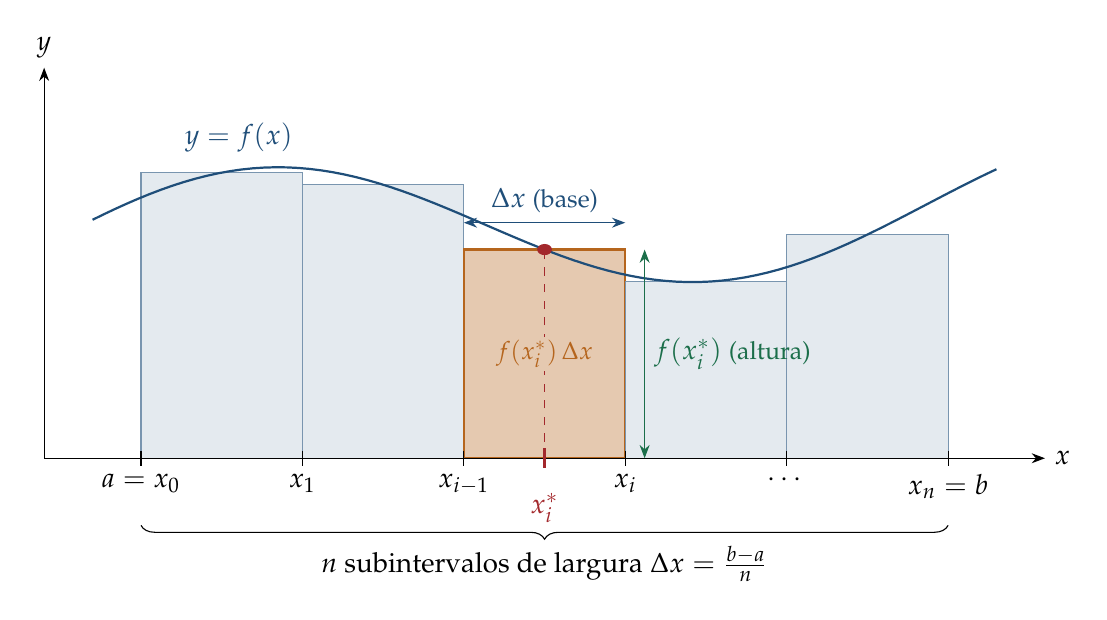
\begin{tikzpicture}[xscale=2.05, yscale=1.55, >=Stealth]
  \def\f#1{(1.75 + 0.55*sin(1.15*#1 r) + 0.06*#1)}
  \def\a{0.6}\def\b{5.6}\def\n{5}
  \pgfmathsetmacro{\dx}{(\b-\a)/\n}
  % retângulos (pontos médios)
  \foreach \i in {1,...,5}{
    \pgfmathsetmacro{\xl}{\a+(\i-1)*\dx}
    \pgfmathsetmacro{\xr}{\a+\i*\dx}
    \pgfmathsetmacro{\xm}{(\xl+\xr)/2}
    \pgfmathsetmacro{\h}{\f{\xm}}
    \ifnum\i=3
      \fill[cSum!35] (\xl,0) rectangle (\xr,\h);
      \draw[cSum, thick] (\xl,0) rectangle (\xr,\h);
    \else
      \fill[azul!12] (\xl,0) rectangle (\xr,\h);
      \draw[azul!60] (\xl,0) rectangle (\xr,\h);
    \fi
  }
  % curva
  \draw[thick, azul, domain=0.3:5.9, samples=80] plot (\x, {\f{\x}});
  \node[azul, above left] at (1.6,{\f{1.6}+0.05}) {$y=f(x)$};
  % eixos
  \draw[->] (0,0) -- (6.2,0) node[right] {$x$};
  \draw[->] (0,0) -- (0,3.2) node[above] {$y$};
  % marcas
  \pgfmathsetmacro{\xl}{\a+2*\dx}\pgfmathsetmacro{\xr}{\a+3*\dx}\pgfmathsetmacro{\xm}{(\xl+\xr)/2}
  \pgfmathsetmacro{\h}{\f{\xm}}
  \foreach \i in {0,...,5}{
    \pgfmathsetmacro{\xx}{\a+\i*\dx}
    \draw (\xx,0.06) -- (\xx,-0.06);
  }
  \node[below] at (\a,-0.05) {$a=x_0$};
  \node[below] at (\b,-0.05) {$x_n=b$};
  \node[below] at (\a+\dx,-0.05) {$x_1$};
  \node[below] at (\xl,-0.05) {$x_{i-1}$};
  \node[below] at (\xr,-0.05) {$x_i$};
  \node[below] at (\a+4*\dx,-0.05) {$\cdots$};
  % ponto amostral
  \draw[cX, thick] (\xm,0.08) -- (\xm,-0.08);
  \node[cX, below, yshift=-9pt] at (\xm,0) {$x_i^*$};
  \draw[cX, dashed] (\xm,0) -- (\xm,\h);
  \fill[cX] (\xm,\h) circle (1.3pt);
  % altura
  \draw[cF, <->] (\xr+0.12,0) -- (\xr+0.12,\h) node[midway, right, cF] {$f(x_i^*)$ \small(altura)};
  % largura
  \draw[cDx, <->] (\xl,\h+0.22) -- (\xr,\h+0.22) node[midway, above, cDx] {$\Delta x$ \small(base)};
  % area label
  \node[cSum, font=\small, fill=cSum!35, inner sep=1pt] at (\xm,\h/2) {$f(x_i^*)\,\Delta x$};
  % chaves
  \draw[decorate, decoration={brace, amplitude=5pt, mirror}] (\a,-0.55) -- (\b,-0.55) node[midway, below, yshift=-4pt] {$n$ subintervalos de largura $\Delta x=\frac{b-a}{n}$};
\end{tikzpicture}
\end{center}

\begin{center}
\small
\renewcommand{\arraystretch}{1.3}
\begin{tabular}{@{}>{\centering\arraybackslash}p{1.8cm}>{\raggedright\arraybackslash}p{6.0cm}>{\raggedright\arraybackslash}p{8.2cm}@{}}
\toprule
\textbf{Símbolo} & \textbf{O que é} & \textbf{Como calcular / como ler}\\
\midrule
$a$, $b$ & extremos do intervalo & a integral ``começa em $a$ e termina em $b$''; $b-a$ é o comprimento total\\
$n$ & número de subintervalos (retângulos) & você escolhe $n$ para \emph{estimar}; na integral, $n\to\infty$\\
\textcolor{cDx}{$\Delta x$} & largura (base) de cada retângulo & $\Delta x=\dfrac{b-a}{n}$ --- comprimento total dividido em $n$ partes iguais\\
$x_0,\dots,x_n$ & as divisões (extremidades dos subintervalos) & $x_i = a+i\,\Delta x$; $x_0=a$, $x_n=b$; o $i$-ésimo subintervalo é $[x_{i-1},x_i]$\\
\textcolor{cX}{$x_i^*$} & ponto amostral: onde medimos a altura & qualquer ponto de $[x_{i-1},x_i]$: esquerda $x_i^*=x_{i-1}$; direita $x_i^*=x_i$; ponto médio $\bar x_i=\dfrac{x_{i-1}+x_i}{2}=a+\big(i-\tfrac12\big)\Delta x$\\
\textcolor{cF}{$f(x_i^*)$} & altura do $i$-ésimo retângulo, \textbf{com sinal} & se $f(x_i^*)<0$ o retângulo fica abaixo do eixo e sua contribuição é negativa\\
\textcolor{cF}{$f(x_i^*)$}\textcolor{cDx}{$\Delta x$} & área (com sinal) do $i$-ésimo retângulo & altura $\times$ base; unidade $=[f]\cdot[x]$\\
\textcolor{cSum}{$\sum_{i=1}^{n}$} & somar os $n$ retângulos & $i=1$ é o primeiro (encostado em $a$), $i=n$ o último (encostado em $b$). Dentro do $\sum$, $n$ é \emph{constante}; $i$ é o que varia\\
\textcolor{cLim}{$\lim_{n\to\infty}$} & mais retângulos, cada vez mais finos & $n\to\infty \Leftrightarrow \Delta x\to 0$; o erro da aproximação vai a zero; o valor do limite é a integral (um \textbf{número})\\
\bottomrule
\end{tabular}
\end{center}

\begin{definicao}[{A notação de Leibniz é a soma de Riemann ``no limite''}]
\[
\textcolor{cLim}{\lim_{n\to\infty}}\textcolor{cSum}{\sum_{i=1}^n} \;\longrightarrow\; \int_a^b
\qquad
\textcolor{cX}{x_i^*} \;\longrightarrow\; x
\qquad
\textcolor{cDx}{\Delta x} \;\longrightarrow\; dx
\qquad
\textcolor{cF}{f(x_i^*)}\textcolor{cDx}{\Delta x} \;\longrightarrow\; f(x)\dx
\]
O $\int$ é um S alongado (de \emph{soma}); $f(x)\dx$ é ``a área de uma fatia infinitamente fina''. O $dx$ não é enfeite: ele diz \emph{qual} variável varia (importa em $\int_a^x f(t)\dt$, Parte 4) e carrega a unidade de $x$. É por isso que a unidade de $\int_a^b f(x)\dx$ é $[f]\times[x]$: (m/s)$\cdot$s $=$ m; (kg/m)$\cdot$m $=$ kg.
\end{definicao}

\subsection{Estimativas: $L_n$, $R_n$, $M_n$ e quem é sub/superestimativa}

\[
L_n=\sum_{i=1}^n f(x_{i-1})\Delta x,\qquad
R_n=\sum_{i=1}^n f(x_i)\Delta x,\qquad
M_n=\sum_{i=1}^n f(\bar x_i)\Delta x .
\]

\begin{geo}[{Sub ou superestimativa? Olhe a monotonia}]
\begin{itemize}[leftmargin=1.4em, itemsep=1pt]
\item $f$ \textbf{crescente} em $[a,b]$: cada retângulo esquerdo fica \emph{dentro} da região e cada direito \emph{sobra} $\Rightarrow$ $L_n\le A\le R_n$.
\item $f$ \textbf{decrescente}: inverte, $R_n\le A\le L_n$.
\item $M_n$ costuma ser a melhor das três (os erros de cada retângulo se compensam parcialmente).
\item Para $f$ monótona, $R_n-L_n=\Delta x\,[f(b)-f(a)]$ (Ex. 5.1.25): os ``degraus'' de diferença entre os dois empilham em um único retângulo de base $\Delta x$ e altura $f(b)-f(a)$. Como $\Delta x\to 0$, $L_n$ e $R_n$ espremem $A$ pelo meio.
\end{itemize}
\end{geo}

\begin{exemplo}[{Exemplo 3.1 --- $f(x)=x^2$ em $[0,1]$, $n=4$ (o exemplo clássico da seção 5.1)}]
$\Delta x=\dfrac{1-0}{4}=\dfrac14$; divisões $x_0=0,\ x_1=\tfrac14,\ x_2=\tfrac12,\ x_3=\tfrac34,\ x_4=1$.

\textbf{Extremidades direitas:}
\[
R_4=\Delta x\big[f(\tfrac14)+f(\tfrac12)+f(\tfrac34)+f(1)\big]
=\frac14\Big[\frac1{16}+\frac4{16}+\frac9{16}+\frac{16}{16}\Big]=\frac14\cdot\frac{30}{16}=\frac{15}{32}=0{,}46875 .
\]
\textbf{Extremidades esquerdas:}
\[
L_4=\frac14\big[f(0)+f(\tfrac14)+f(\tfrac12)+f(\tfrac34)\big]
=\frac14\Big[0+\frac1{16}+\frac4{16}+\frac9{16}\Big]=\frac14\cdot\frac{14}{16}=\frac{7}{32}=0{,}21875 .
\]
\textbf{Pontos médios} $\bar x_i=\tfrac18,\tfrac38,\tfrac58,\tfrac78$:
\[
M_4=\frac14\Big[\frac1{64}+\frac9{64}+\frac{25}{64}+\frac{49}{64}\Big]=\frac14\cdot\frac{84}{64}=\frac{21}{64}=0{,}328125 .
\]
Como $x^2$ é crescente em $[0,1]$: $L_4=0{,}219<A<0{,}469=R_4$. Valor exato (Ex.~3.3 e TFC): $A=\tfrac13=0{,}3333\ldots$ --- $M_4$ já erra só $0{,}005$. Conferindo a fórmula da diferença: $R_4-L_4=\tfrac14[f(1)-f(0)]=\tfrac14$ \ok.

\begin{center}
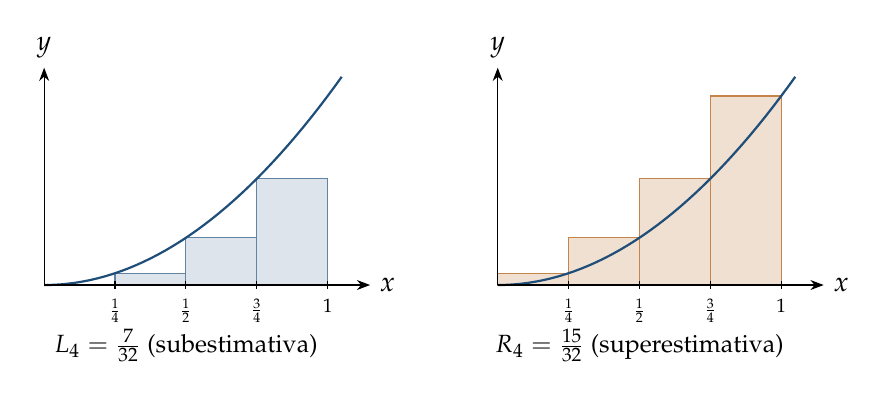
\begin{tikzpicture}[xscale=3.6, yscale=2.4, >=Stealth]
  % L4
  \begin{scope}
    \foreach \i in {1,...,4}{
      \pgfmathsetmacro{\xl}{(\i-1)/4}\pgfmathsetmacro{\xr}{\i/4}\pgfmathsetmacro{\h}{\xl*\xl}
      \fill[azul!15] (\xl,0) rectangle (\xr,\h);
      \draw[azul!70] (\xl,0) rectangle (\xr,\h);
    }
    \draw[thick, azul, domain=0:1.05, samples=40] plot (\x,{\x*\x});
    \draw[->] (0,0) -- (1.15,0) node[right] {$x$};
    \draw[->] (0,0) -- (0,1.15) node[above] {$y$};
    \foreach \x/\l in {0.25/\frac14, 0.5/\frac12, 0.75/\frac34, 1/1}{\draw (\x,0.02)--(\x,-0.02) node[below,font=\scriptsize] {$\l$};}
    \node[font=\small] at (0.5,-0.32) {$L_4=\tfrac{7}{32}$ (subestimativa)};
  \end{scope}
  % R4
  \begin{scope}[shift={(1.6,0)}]
    \foreach \i in {1,...,4}{
      \pgfmathsetmacro{\xl}{(\i-1)/4}\pgfmathsetmacro{\xr}{\i/4}\pgfmathsetmacro{\h}{\xr*\xr}
      \fill[cSum!20] (\xl,0) rectangle (\xr,\h);
      \draw[cSum!80] (\xl,0) rectangle (\xr,\h);
    }
    \draw[thick, azul, domain=0:1.05, samples=40] plot (\x,{\x*\x});
    \draw[->] (0,0) -- (1.15,0) node[right] {$x$};
    \draw[->] (0,0) -- (0,1.15) node[above] {$y$};
    \foreach \x/\l in {0.25/\frac14, 0.5/\frac12, 0.75/\frac34, 1/1}{\draw (\x,0.02)--(\x,-0.02) node[below,font=\scriptsize] {$\l$};}
    \node[font=\small] at (0.5,-0.32) {$R_4=\tfrac{15}{32}$ (superestimativa)};
  \end{scope}
\end{tikzpicture}
\end{center}
\end{exemplo}

\begin{exemplo}[{Exemplo 3.2 --- estimando distância a partir de velocidades (5.1.11 / 5.4.75)}]
Leituras de velocidade de um carro: $t=0,10,20,30$ s $\to$ $v=0,\ 6,\ 10,\ 12$ m/s. Estime a distância nos 30 s.

Aqui $f=v$, $\Delta t = 10$ s e $n=3$. Esquerda: $L_3=(0+6+10)\cdot 10=160$ m. Direita: $R_3=(6+10+12)\cdot 10=280$ m. Se $v$ é crescente no período, $160\le d\le 280$; uma estimativa melhor é a média, $220$ m. Unidade: (m/s)$\cdot$s $=$ m --- a unidade da integral é sempre altura $\times$ base.

\textbf{Leitura:} ``distância $=$ área sob a curva da velocidade'' é o primeiro caso do Teorema da Variação Total (Parte 4).
\end{exemplo}

\subsection{Uma soma de Riemann com $f$ mudando de sinal (5.2.1--3)}

\begin{exemplo}[{Exemplo 3.3 --- $f(x)=x^2-4$ em $[0,3]$, $n=6$, pontos médios (questão 5.2.3)}]
$\Delta x=\dfrac{3-0}{6}=\dfrac12$. Divisões $0,\ \tfrac12,\ 1,\ \tfrac32,\ 2,\ \tfrac52,\ 3$; pontos médios $\bar x_i = \tfrac14,\tfrac34,\tfrac54,\tfrac74,\tfrac94,\tfrac{11}4$.

\begin{center}
\small
\begin{tabular}{@{}c|cccccc@{}}
$i$ & 1 & 2 & 3 & 4 & 5 & 6\\
\hline
$\bar x_i$ & $0{,}25$ & $0{,}75$ & $1{,}25$ & $1{,}75$ & $2{,}25$ & $2{,}75$\\
$\bar x_i^{\,2}$ & $0{,}0625$ & $0{,}5625$ & $1{,}5625$ & $3{,}0625$ & $5{,}0625$ & $7{,}5625$\\
$f(\bar x_i)=\bar x_i^{\,2}-4$ & $-3{,}9375$ & $-3{,}4375$ & $-2{,}4375$ & $-0{,}9375$ & $1{,}0625$ & $3{,}5625$\\
$f(\bar x_i)\Delta x$ & $-1{,}96875$ & $-1{,}71875$ & $-1{,}21875$ & $-0{,}46875$ & $0{,}53125$ & $1{,}78125$\\
\end{tabular}
\end{center}
\begin{align*}
M_6=\sum_{i=1}^6 f(\bar x_i)\Delta x &= \frac12\big(-3{,}9375-3{,}4375-2{,}4375-0{,}9375+1{,}0625+3{,}5625\big)\\
&=\frac12(-6{,}125)=-3{,}0625 .
\end{align*}
\textbf{O que a soma representa:} os quatro primeiros retângulos estão \emph{abaixo} do eixo (contribuem negativo) e os dois últimos \emph{acima}. $M_6$ é (área dos retângulos acima) $-$ (área dos retângulos abaixo) $= 2{,}3125-5{,}375=-3{,}0625$. \textbf{Não} é ``a área da região'' --- é uma aproximação da \emph{área líquida com sinal}, isto é, de $\int_0^3(x^2-4)\dx$.

\begin{center}
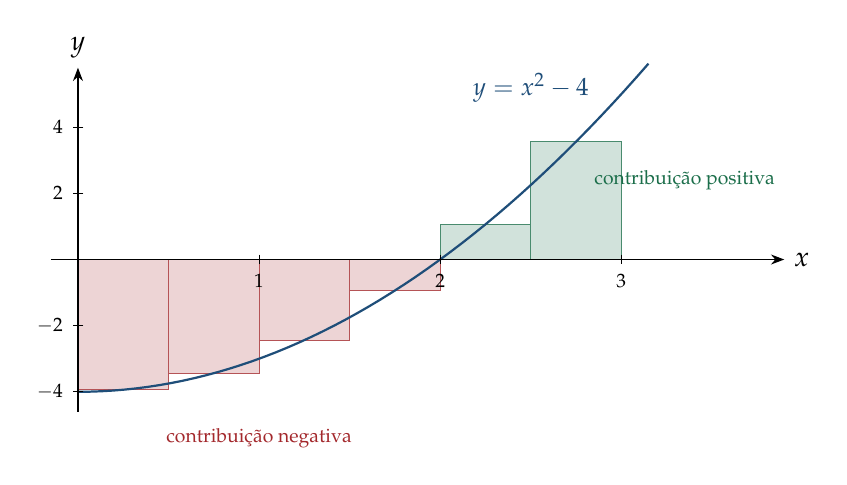
\begin{tikzpicture}[xscale=2.3, yscale=0.42, >=Stealth]
  \foreach \i in {1,...,6}{
    \pgfmathsetmacro{\xl}{(\i-1)/2}\pgfmathsetmacro{\xr}{\i/2}\pgfmathsetmacro{\xm}{(\xl+\xr)/2}
    \pgfmathsetmacro{\h}{\xm*\xm-4}
    \ifdim \h pt<0pt
      \fill[vermelho!20] (\xl,0) rectangle (\xr,\h); \draw[vermelho!80] (\xl,0) rectangle (\xr,\h);
    \else
      \fill[verde!20] (\xl,0) rectangle (\xr,\h); \draw[verde!80] (\xl,0) rectangle (\xr,\h);
    \fi
  }
  \draw[thick, azul, domain=0:3.15, samples=50] plot (\x,{\x*\x-4});
  \draw[->] (-0.15,0) -- (3.9,0) node[right] {$x$};
  \draw[->] (0,-4.6) -- (0,5.8) node[above] {$y$};
  \foreach \x in {1,2,3}{\draw (\x,0.15)--(\x,-0.15) node[below,font=\scriptsize] {$\x$};}
  \foreach \y in {-4,-2,2,4}{\draw (0.03,\y)--(-0.03,\y) node[left,font=\scriptsize] {$\y$};}
  \node[azul, font=\small] at (2.5,5.2) {$y=x^2-4$};
  \node[vermelho, font=\scriptsize, align=center] at (1.0,-5.4) {contribuição negativa};
  \node[verde, font=\scriptsize, align=center] at (3.35,2.4) {contribuição positiva};
\end{tikzpicture}
\end{center}
\end{exemplo}

\begin{definicao}[{Integral definida $=$ área líquida (com sinal)}]
\[
\int_a^b f(x)\dx = (\text{área das partes \emph{acima} do eixo }x) - (\text{área das partes \emph{abaixo}}).
\]
Se $f\ge 0$ em $[a,b]$, a integral é a área. Se $f$ muda de sinal, a integral pode ser zero ou negativa mesmo com região ``grande''. A \emph{área geométrica} total é $\int_a^b |f(x)|\dx$ --- exige separar nos zeros de $f$ (mesma ideia de ``distância percorrida'' na Parte 4).
\end{definicao}

\subsection{Fórmulas de somatório (para calcular o limite exato)}

\begin{definicao}[{Somas de potências e regras do $\sum$}]
\[
\sum_{i=1}^n c = nc,\qquad
\sum_{i=1}^n i=\frac{n(n+1)}{2},\qquad
\sum_{i=1}^n i^2=\frac{n(n+1)(2n+1)}{6},\qquad
\sum_{i=1}^n i^3=\Big[\frac{n(n+1)}{2}\Big]^2 .
\]
\[
\sum_{i=1}^n (c\,a_i+b_i)=c\sum_{i=1}^n a_i+\sum_{i=1}^n b_i \qquad\text{(tudo que não depende de $i$ sai do somatório --- inclusive $n$)}.
\]
\end{definicao}

\subsection{Calcular a integral pela definição (Teorema 4) --- questões 5.2.27--34}

\begin{metodo}[{Roteiro em seis passos}]
\begin{enumerate}[leftmargin=1.6em, itemsep=1pt]
\item Escreva $\Delta x=\frac{b-a}{n}$ e $x_i=a+i\Delta x$.
\item Calcule $f(x_i)$: substitua $x_i$ na função e \emph{expanda} até ficar um polinômio em $i$ com coeficientes em $n$.
\item Monte $R_n=\sum f(x_i)\Delta x$ e distribua; tire para fora do $\sum$ tudo que não depende de $i$.
\item Substitua as fórmulas de $\sum i$, $\sum i^2$, $\sum i^3$, $\sum 1$.
\item Simplifique cancelando potências de $n$; escreva em termos de $\frac1n$.
\item Faça $n\to\infty$: todo termo com $\frac1n$, $\frac1{n^2}$, \dots\ vai a zero.
\end{enumerate}
\end{metodo}

\begin{exemplo}[{Exemplo 3.4 --- $\displaystyle\int_0^3 (x^2-4)\dx$ pela definição (a mesma função do Ex.~3.3)}]
\textbf{1.} $\Delta x=\dfrac{3-0}{n}=\dfrac3n$, \quad $x_i=0+i\cdot\dfrac3n=\dfrac{3i}{n}$.

\textbf{2.} $f(x_i)=\Big(\dfrac{3i}{n}\Big)^2-4=\dfrac{9i^2}{n^2}-4$.

\textbf{3.} $R_n=\displaystyle\sum_{i=1}^n\Big(\frac{9i^2}{n^2}-4\Big)\frac3n
=\sum_{i=1}^n\frac{27i^2}{n^3}-\sum_{i=1}^n\frac{12}{n}
=\frac{27}{n^3}\sum_{i=1}^n i^2-\frac{12}{n}\sum_{i=1}^n 1 .$

\textbf{4.} $=\dfrac{27}{n^3}\cdot\dfrac{n(n+1)(2n+1)}{6}-\dfrac{12}{n}\cdot n$.

\textbf{5.} $=\dfrac{27}{6}\cdot\dfrac{(n+1)(2n+1)}{n^2}-12=\dfrac92\cdot\dfrac{n+1}{n}\cdot\dfrac{2n+1}{n}-12=\dfrac92\Big(1+\dfrac1n\Big)\Big(2+\dfrac1n\Big)-12$.

\textbf{6.} $\displaystyle\int_0^3(x^2-4)\dx=\lim_{n\to\infty}R_n=\frac92\cdot 1\cdot 2-12=9-12=\boxed{-3}$.

\textbf{Verificação pelo TFC2 (Parte 4):} $\Big[\dfrac{x^3}{3}-4x\Big]_0^3=(9-12)-0=-3$ \ok.

\textbf{Verificação geométrica:} $x^2-4<0$ em $[0,2)$ e $>0$ em $(2,3]$. Área abaixo: $\int_0^2(4-x^2)\dx=8-\tfrac83=\tfrac{16}{3}$. Área acima: $\int_2^3(x^2-4)\dx=(9-12)-(\tfrac83-8)=\tfrac73$. Líquida: $\tfrac73-\tfrac{16}3=-3$ \ok. E o $M_6=-3{,}0625$ do Ex.~3.3 erra por só $0{,}06$.
\end{exemplo}

\begin{armadilha}[{Erros que aparecem nesse cálculo}]
\begin{itemize}[leftmargin=1.4em, itemsep=1pt]
\item Tratar $n$ como se variasse dentro do $\sum$ (ou $i$ como constante). Dentro do somatório, \textbf{$n$ é fixo}; só $i$ corre de $1$ a $n$.
\item Esquecer de multiplicar por $\Delta x$ (a soma fica sem a base dos retângulos e a unidade fica errada).
\item $\sum_{i=1}^n 4 = 4n$, não $4$. E $\sum_{i=1}^n \frac{c}{n}=c$.
\item Esquecer o $a$ em $x_i=a+i\Delta x$ quando $a\neq 0$: para $[1,3]$ com $n$ partes, $x_i=1+\frac{2i}{n}$.
\item Escrever $\lim$ na frente só na última linha. Enquanto há $n$, é $R_n$; o $\lim$ entra quando você vai avaliar.
\end{itemize}
\end{armadilha}

\subsection{A definição geral e quando a integral existe}

\begin{definicao}[{Definição 2 e Teorema 3 da seção 5.2}]
Para $f$ definida em $[a,b]$, divida $[a,b]$ em $n$ subintervalos de largura $\Delta x$ e escolha pontos amostrais $x_i^*$ \emph{quaisquer} em $[x_{i-1},x_i]$. A \textbf{integral definida} é
\[
\int_a^b f(x)\dx=\lim_{n\to\infty}\sum_{i=1}^n f(x_i^*)\Delta x
\]
desde que o limite exista \emph{e dê o mesmo valor para toda escolha dos $x_i^*$}. Nesse caso $f$ é \textbf{integrável}.

\textbf{Teorema.} Se $f$ é contínua em $[a,b]$, ou tem apenas um número finito de descontinuidades de salto, então $f$ é integrável em $[a,b]$.

Vocabulário: $f$ é o \emph{integrando}; $a$ e $b$ são os \emph{limites de integração}; a variável é \emph{muda}: $\int_a^b f(x)\dx=\int_a^b f(t)\dt=\int_a^b f(r)\,dr$.
\end{definicao}

Se $f$ é integrável, \emph{qualquer} escolha de pontos amostrais dá o mesmo limite --- por isso podemos usar sempre extremidades direitas para calcular (Teorema 4) e pontos médios para estimar (Regra do Ponto Médio). O que muda com a escolha é só a velocidade de convergência, não o valor.

\subsection{Traduzir: limite $\leftrightarrow$ integral (5.2.19--22, 25--26; 5.1.16--23; 5.3.85--86)}

\begin{metodo}[{Como reconhecer uma soma de Riemann}]
Dado $\displaystyle\lim_{n\to\infty}\sum_{i=1}^n(\cdots)$:
\begin{enumerate}[leftmargin=1.6em, itemsep=1pt]
\item Ache o fator que \textbf{não depende de $i$} e é proporcional a $\frac1n$: é $\Delta x$; então $b-a=n\Delta x$.
\item Ache a expressão da forma $a+i\Delta x$ dentro da função: é $x_i$; ela revela $a$ (e $b=a+n\Delta x$).
\item O que sobra, escrito em função de $x_i$, é $f(x_i)$. Troque $x_i\to x$, $\Delta x\to dx$, $\lim\sum\to\int_a^b$.
\end{enumerate}
Caso especial frequente: se aparece $\frac{i}{n}$ e o fator é $\frac1n$, então $\Delta x=\frac1n$, $x_i=\frac in$, intervalo $[0,1]$.
\end{metodo}

\begin{exemplo}[{Exemplo 3.5 --- de limite para integral (5.2.19--22)}]
$\displaystyle\lim_{n\to\infty}\sum_{i=1}^n\big[(x_i^*)^3+x_i^*\sen x_i^*\big]\Delta x$ em $[0,\pi]$.

O padrão é literal: $f(x)=x^3+x\sen x$, $a=0$, $b=\pi$. Logo o limite é $\displaystyle\int_0^{\pi}(x^3+x\sen x)\dx$.
\end{exemplo}

\begin{exemplo}[{Exemplo 3.6 --- limite ``escondido'' em $[0,1]$ (questão 5.3.85)}]
$\displaystyle\lim_{n\to\infty}\sum_{i=1}^n\Big(\frac{i^4}{n^5}+\frac{i}{n^2}\Big)$.

\textbf{Reconhecer:} $\dfrac{i^4}{n^5}=\Big(\dfrac in\Big)^4\cdot\dfrac1n$ e $\dfrac{i}{n^2}=\Big(\dfrac in\Big)\cdot\dfrac1n$. O fator comum é $\dfrac1n=\Delta x$ e $x_i=\dfrac in$ $\Rightarrow$ $a=0$, $b=1$, $f(x)=x^4+x$.
\[
\lim_{n\to\infty}\sum_{i=1}^n\big[x_i^4+x_i\big]\Delta x=\int_0^1(x^4+x)\dx=\Big[\frac{x^5}{5}+\frac{x^2}{2}\Big]_0^1=\frac15+\frac12=\frac{7}{10}.
\]
\end{exemplo}

\begin{exemplo}[{Exemplo 3.7 --- soma escrita por extenso (questão 5.3.86)}]
$\displaystyle\lim_{n\to\infty}\frac1n\Big(\sqrt{\tfrac1n}+\sqrt{\tfrac2n}+\sqrt{\tfrac3n}+\cdots+\sqrt{\tfrac nn}\Big)$.

Reescreva com $\sum$: $\displaystyle\lim_{n\to\infty}\sum_{i=1}^n\sqrt{\frac in}\cdot\frac1n$. Então $\Delta x=\frac1n$, $x_i=\frac in$, $[0,1]$, $f(x)=\sqrt x$:
\[
=\int_0^1\sqrt x\dx=\int_0^1 x^{1/2}\dx=\Big[\frac{x^{3/2}}{3/2}\Big]_0^1=\frac23 .
\]
\textbf{Leitura:} o limite é a área sob $y=\sqrt x$ de $0$ a $1$ --- dois terços do quadrado unitário.
\end{exemplo}

\begin{exemplo}[{Exemplo 3.8 --- identificar a região sem calcular (5.1.20--23)}]
$\displaystyle\lim_{n\to\infty}\sum_{i=1}^n\frac{\pi}{4n}\,\tg\!\Big(\frac{i\pi}{4n}\Big)$.

$\Delta x=\dfrac{\pi}{4n}$ $\Rightarrow$ $b-a=\dfrac\pi4$. \; $x_i=\dfrac{i\pi}{4n}=0+i\Delta x$ $\Rightarrow$ $a=0$, $b=\dfrac\pi4$. \; $f(x)=\tg x$.

Região: sob $y=\tg x$, de $x=0$ a $x=\pi/4$. (Não calcule; o enunciado pede só a região.)
\end{exemplo}

\begin{exemplo}[{Exemplo 3.9 --- de integral para limite (5.2.25--26)}]
Escreva $\displaystyle\int_1^3\sqrt{4+x^2}\dx$ como limite de somas de Riemann com extremidades direitas.

$\Delta x=\dfrac{3-1}{n}=\dfrac2n$, \; $x_i=1+\dfrac{2i}{n}$:
\[
\int_1^3\sqrt{4+x^2}\dx=\lim_{n\to\infty}\sum_{i=1}^n\sqrt{4+\Big(1+\frac{2i}{n}\Big)^2}\cdot\frac2n .
\]
Observação: a leitura de um limite como integral não é única (o mesmo limite pode ser lido em $[0,2]$ com outra $f$, reescalando). Qualquer escolha coerente é aceita --- o que não pode é $\Delta x$ e $x_i$ virem de intervalos diferentes.
\end{exemplo}

\subsection{Calcular integrais por áreas (5.2.41--46)}

Quando o gráfico é feito de retas e arcos de círculo, a integral sai da geometria --- sem primitiva. Lembre: contribuição positiva acima do eixo, negativa abaixo.

\begin{center}
\small
\begin{tabular}{@{}ll@{}}
\toprule
\textbf{Integrando} & \textbf{Figura e área}\\
\midrule
constante $c$ & retângulo: $c\,(b-a)$\\
$mx+k$ (não muda de sinal) & trapézio: $\dfrac{f(a)+f(b)}{2}\,(b-a)$\\
$\sqrt{r^2-x^2}$ em $[-r,r]$ & semicírculo: $\dfrac{\pi r^2}{2}$ (em $[0,r]$: quarto de círculo $\dfrac{\pi r^2}{4}$)\\
$|x-c|$ & dois triângulos com vértice em $x=c$\\
reta que cruza o eixo & dois triângulos, um positivo e um negativo\\
\bottomrule
\end{tabular}
\end{center}

\begin{exemplo}[{Exemplo 3.10 --- três integrais por áreas}]
\textbf{(a)} $\displaystyle\int_1^4(2x-1)\dx$. Reta com $f(1)=1$ e $f(4)=7$, positiva em $[1,4]$: trapézio de bases $1$ e $7$ e altura $3$: $\dfrac{1+7}{2}\cdot 3=12$. Conferindo: $[x^2-x]_1^4=(16-4)-(1-1)=12$ \ok.

\textbf{(b)} $\displaystyle\int_{-3}^{3}\big(1+\sqrt{9-x^2}\big)\dx=\int_{-3}^3 1\dx+\int_{-3}^3\sqrt{9-x^2}\dx = 6+\frac{\pi\cdot 3^2}{2}=6+\frac{9\pi}{2}$ (retângulo $6\times1$ mais semicírculo de raio $3$).

\textbf{(c)} $\displaystyle\int_0^{10}|x-5|\dx$: triângulo de $0$ a $5$ (base 5, altura 5) e outro de $5$ a $10$, ambos acima do eixo: $2\cdot\dfrac{5\cdot5}{2}=25$.

\textbf{(d)} $\displaystyle\int_{-2}^{4}(6-2x)\dx$: a reta zera em $x=3$. Triângulo acima em $[-2,3]$: base $5$, altura $f(-2)=10$, área $25$. Triângulo abaixo em $[3,4]$: base $1$, altura $|f(4)|=2$, área $1$. Integral $=25-1=24$. Conferindo: $[6x-x^2]_{-2}^4=(24-16)-(-12-4)=8+16=24$ \ok.
\end{exemplo}

\subsection{Propriedades da integral definida (5.2.53--62)}

\begin{definicao}[{Propriedades}]
\begin{multicols}{2}
\begin{enumerate}[leftmargin=1.6em, itemsep=1pt]
\item $\displaystyle\int_a^a f\dx=0$
\item $\displaystyle\int_b^a f\dx=-\int_a^b f\dx$
\item $\displaystyle\int_a^b c\dx=c(b-a)$
\item $\displaystyle\int_a^b(cf\pm g)\dx=c\int_a^b f\dx\pm\int_a^b g\dx$
\item $\displaystyle\int_a^c f\dx+\int_c^b f\dx=\int_a^b f\dx$ (para qualquer $c$)
\item $f\ge0$ em $[a,b]\Rightarrow\displaystyle\int_a^b f\dx\ge0$
\item $f\ge g$ em $[a,b]\Rightarrow\displaystyle\int_a^b f\dx\ge\int_a^b g\dx$
\item $m\le f\le M$ em $[a,b]\Rightarrow m(b-a)\le\displaystyle\int_a^b f\dx\le M(b-a)$
\end{enumerate}
\end{multicols}
\end{definicao}

\begin{exemplo}[{Exemplo 3.11 --- usando as propriedades}]
\textbf{(a)} Se $\int_0^9 f\dx=37$ e $\int_0^9 g\dx=16$: $\displaystyle\int_0^9[2f+3g]\dx=2(37)+3(16)=122$.

\textbf{(b)} Se $\int_1^5 f\dx=12$ e $\int_4^5 f\dx=3{,}6$: $\displaystyle\int_1^4 f\dx=12-3{,}6=8{,}4$ (propriedade 5).

\textbf{(c)} Sabendo que $\int_0^1 x^2\dx=\frac13$: $\displaystyle\int_0^1(5-6x^2)\dx=5\cdot1-6\cdot\frac13=3$.

\textbf{(d)} Estime $\int_0^1 e^{-x^2}\dx$: $e^{-x^2}$ é decrescente em $[0,1]$, máximo $M=e^0=1$, mínimo $m=e^{-1}$. Propriedade 8: $e^{-1}\le\int_0^1 e^{-x^2}\dx\le1$, ou seja, entre $0{,}37$ e $1$. (A integral está entre o retângulo baixo e o quadrado.)
\end{exemplo}

\begin{exercicios}[{Exercícios similares --- Parte 3}]
\begin{enumerate}[leftmargin=1.6em, itemsep=2pt, label=\textbf{3.\arabic*}]
\item $f(x)=x^3$ em $[0,2]$, $n=4$. Calcule $R_4$ e $L_4$, diga qual é sub/superestimativa e por quê. (Exato: $4$.)
\item $f(x)=1/x$ em $[1,2]$, $n=4$, extremidades direitas (questão 5.1.3). Sub ou super? Repita com esquerdas.
\item Calcule $\displaystyle\int_1^3(x^2+1)\dx$ pela definição (Teorema 4). Confira pelo TFC.
\item Expresse como integral: (a) $\displaystyle\lim_{n\to\infty}\sum_{i=1}^n\big[5(x_i^*)^3-4x_i^*\big]\Delta x$ em $[2,7]$; (b) $\displaystyle\lim_{n\to\infty}\sum_{i=1}^n\frac3n\sqrt{1+\frac{3i}{n}}$ --- e calcule (b).
\item Determine a região cuja área é $\displaystyle\lim_{n\to\infty}\sum_{i=1}^n\frac2n\Big(5+\frac{2i}{n}\Big)^{10}$.
\item Por áreas: (a) $\displaystyle\int_0^4|x-1|\dx$; \;(b) $\displaystyle\int_{-2}^2\sqrt{4-x^2}\dx$; \;(c) $\displaystyle\int_0^3(2x-4)\dx$.
\item Escreva $\displaystyle\int_0^2 e^{x}\dx$ como limite de somas de Riemann com extremidades direitas (não calcule).
\item Use a propriedade 8 para mostrar que $\displaystyle 2\le\int_{-1}^1\sqrt{1+x^2}\dx\le 2\sqrt2$.
\end{enumerate}
\end{exercicios}

\section[TFC (5.3) e Teorema da Variação Total (5.4)]{O Teorema Fundamental do Cálculo (5.3) e o Teorema da Variação Total (5.4)}

\subsection{TFC1 --- a função ``área até aqui'' e sua derivada}

\begin{definicao}[{TFC, Parte 1}]
Se $f$ é contínua em $[a,b]$, a função
\[
g(x)=\int_a^x f(t)\dt,\qquad a\le x\le b,
\]
é contínua em $[a,b]$, derivável em $(a,b)$ e
\[
g'(x)=f(x)\qquad\text{ou seja}\qquad \frac{d}{dx}\int_a^x f(t)\dt=f(x).
\]
\end{definicao}

\begin{geo}[{Por que a derivada da área é a altura}]
$g(x)$ é a área sob $f$ de $a$ até $x$ (``área acumulada até aqui''). Ao avançar de $x$ para $x+h$, a área ganha uma faixa fina de largura $h$ e altura $\approx f(x)$:
\[
g(x+h)-g(x)\approx f(x)\,h
\quad\Longrightarrow\quad
\frac{g(x+h)-g(x)}{h}\approx f(x)
\quad\xrightarrow{\;h\to0\;}\quad g'(x)=f(x).
\]
\begin{center}
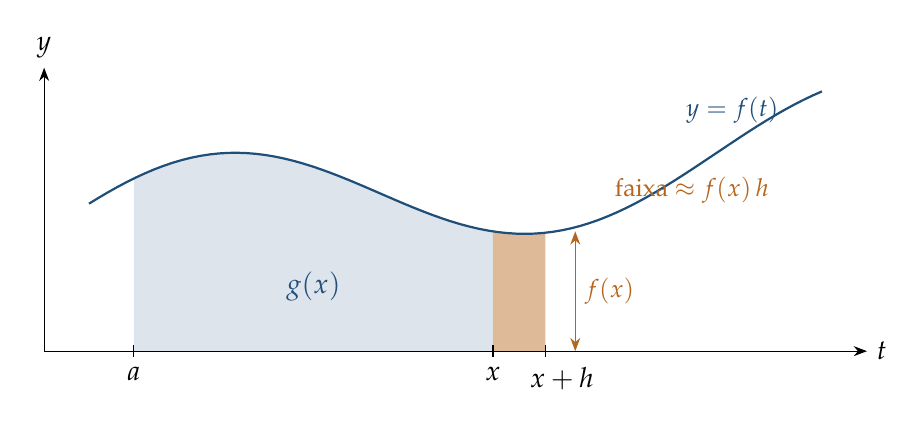
\begin{tikzpicture}[xscale=1.9, yscale=1.5, >=Stealth]
  \def\f#1{(1.0 + 0.5*sin(1.4*#1 r) + 0.15*#1)}
  \fill[azul!15, domain=0.6:3.0, samples=40] plot (\x,{\f{\x}}) -- (3.0,0) -- (0.6,0) -- cycle;
  \fill[cSum!45, domain=3.0:3.35, samples=10] plot (\x,{\f{\x}}) -- (3.35,0) -- (3.0,0) -- cycle;
  \draw[thick, azul, domain=0.3:5.2, samples=80] plot (\x,{\f{\x}});
  \draw[->] (0,0) -- (5.5,0) node[right] {$t$};
  \draw[->] (0,0) -- (0,2.4) node[above] {$y$};
  \draw (0.6,0.05)--(0.6,-0.05) node[below] {$a$};
  \draw (3.0,0.05)--(3.0,-0.05) node[below] {$x$};
  \draw (3.35,0.05)--(3.35,-0.05) node[below, xshift=6pt] {$x+h$};
  \node[azul] at (1.8,0.55) {$g(x)$};
  \pgfmathsetmacro{\hh}{\f{3.0}}
  \draw[cSum, <->] (3.55,0) -- (3.55,\hh) node[midway, right, cSum, font=\small] {$f(x)$};
  \node[azul, font=\small, above] at (4.6,{(1.0 + 0.5*sin(1.4*4.6 r) + 0.15*4.6)+0.08}) {$y=f(t)$};
  \node[cSum, font=\small, align=left, anchor=west] at (3.75,{(1.0 + 0.5*sin(1.4*3.0 r) + 0.15*3.0)+0.35}) {faixa $\approx f(x)\,h$};
\end{tikzpicture}
\end{center}
Observação: a variável de integração $t$ é ``muda'' (interna). $g$ depende só de $x$, que aparece no limite superior. O limite inferior $a$ não aparece na derivada: ele só desloca $g$ por uma constante.
\end{geo}

\begin{definicao}[{Lendo o gráfico de $g(x)=\int_a^x f(t)\dt$ a partir do gráfico de $f$ (5.3.2--4, 83--84)}]
Como $g'=f$ e $g''=f'$:
\begin{itemize}[leftmargin=1.4em, itemsep=1pt]
\item $g(a)=0$ (área de largura zero).
\item $g$ cresce onde $f>0$ (está somando área) e decresce onde $f<0$ (subtraindo).
\item $g$ tem máximo local onde $f$ passa de $+$ para $-$; mínimo local onde passa de $-$ para $+$.
\item $g$ é côncava para cima onde $f$ é crescente, para baixo onde $f$ é decrescente.
\item $g'(c)=f(c)$: a inclinação de $g$ em $c$ é a \emph{altura} de $f$ em $c$. Ex.: se $f(3)=0$ com $f$ mudando de sinal, $g$ tem tangente horizontal em $3$.
\end{itemize}
\end{definicao}

\begin{definicao}[{TFC1 com regra da cadeia --- os três formatos}]
Para $u$ e $v$ deriváveis e $f$ contínua:
\[
\frac{d}{dx}\int_a^{u(x)}f(t)\dt=f\big(u(x)\big)\,u'(x),
\qquad
\frac{d}{dx}\int_{u(x)}^{b}f(t)\dt=-f\big(u(x)\big)\,u'(x),
\]
\[
\frac{d}{dx}\int_{u(x)}^{v(x)}f(t)\dt=f\big(v(x)\big)\,v'(x)-f\big(u(x)\big)\,u'(x).
\]
Origem: $\int_a^{u(x)}f\dt=g(u(x))$ com $g(y)=\int_a^y f\dt$; a regra da cadeia dá $g'(u)\,u'=f(u)\,u'$. O segundo caso é o primeiro com a propriedade $\int_u^b=-\int_b^u$. O terceiro é a soma dos dois, separando em um ponto qualquer.
\end{definicao}

\begin{exemplo}[{Exemplo 4.1 --- as questões 5.3.9, 5.3.10, 5.3.13, 5.3.17, 5.3.19 e o Exemplo 4 do livro}]
\begin{enumerate}[leftmargin=1.6em, itemsep=3pt, label=(\alph*)]
\item $g(x)=\displaystyle\int_1^x\ln(1+t^2)\dt$ \;$\Rightarrow$\; $g'(x)=\ln(1+x^2)$. (Limite superior é $x$ puro: troque $t$ por $x$.)
\item $\dfrac{d}{dx}\displaystyle\int_1^{x^4}\sec t\dt$: $u=x^4$, $u'=4x^3$ \;$\Rightarrow$\; $\sec(x^4)\cdot4x^3$.
\item $F(x)=\displaystyle\int_x^0\sqrt{1+\sec t}\dt=-\int_0^x\sqrt{1+\sec t}\dt$ \;$\Rightarrow$\; $F'(x)=-\sqrt{1+\sec x}$.
\item $y=\displaystyle\int_1^{3x+2}\frac{t}{1+t^3}\dt$: $u=3x+2$, $u'=3$ \;$\Rightarrow$\; $y'=\dfrac{3x+2}{1+(3x+2)^3}\cdot3$.
\item $y=\displaystyle\int_{\sqrt x}^{\pi/4}\theta\tg\theta\,d\theta$: limite inferior variável, $u=\sqrt x$, $u'=\dfrac{1}{2\sqrt x}$:
\[
y'=-\big(\sqrt x\,\tg\sqrt x\big)\cdot\frac{1}{2\sqrt x}=-\frac{\tg\sqrt x}{2}.
\]
\item $h(x)=\displaystyle\int_{2x}^{x^2}\sen(t^2)\dt$ \;$\Rightarrow$\; $h'(x)=\sen\big((x^2)^2\big)\cdot 2x-\sen\big((2x)^2\big)\cdot2=2x\sen(x^4)-2\sen(4x^2)$.
\end{enumerate}
Em nenhum item você precisa (ou consegue) achar a primitiva do integrando. É esse o ponto do TFC1.
\end{exemplo}

\begin{exemplo}[{Exemplo 4.2 --- ``encontre $f$ e $a$'' (questão 5.3.93, favorita de prova)}]
Encontre $f$ e $a$ tais que $\displaystyle 6+\int_a^x\frac{f(t)}{t^2}\dt=2\sqrt x$ para todo $x>0$.

\textbf{Derive os dois lados} (TFC1 à esquerda, tabela à direita): $\dfrac{f(x)}{x^2}=\dfrac{1}{\sqrt x}$ \;$\Rightarrow$\; $f(x)=\dfrac{x^2}{\sqrt x}=x^{3/2}$.

\textbf{Faça $x=a$} (a integral zera): $6+0=2\sqrt a$ \;$\Rightarrow$\; $\sqrt a=3$ \;$\Rightarrow$\; $a=9$.

\textbf{Verificação:} $\displaystyle\int_9^x\frac{t^{3/2}}{t^2}\dt=\int_9^x t^{-1/2}\dt=\big[2\sqrt t\big]_9^x=2\sqrt x-6$; somando $6$ dá $2\sqrt x$ \ok.
\end{exemplo}

\subsection{TFC2 --- calcular integrais definidas com uma primitiva}

\begin{definicao}[{TFC, Parte 2}]
Se $f$ é contínua em $[a,b]$ e $F$ é \emph{qualquer} primitiva de $f$ ($F'=f$), então
\[
\int_a^b f(x)\dx=F(b)-F(a)\;=\;\Big[F(x)\Big]_a^b .
\]
O $C$ some: $(F(b)+C)-(F(a)+C)=F(b)-F(a)$. Por isso, em integrais definidas, não se escreve $C$.

\textbf{As duas partes juntas} dizem que derivar e integrar são operações inversas:
$\dfrac{d}{dx}\displaystyle\int_a^x f(t)\dt=f(x)$ \;e\; $\displaystyle\int_a^x F'(t)\dt=F(x)-F(a)$.
\end{definicao}

\begin{metodo}[{Roteiro para $\int_a^b f(x)\dx$}]
\begin{enumerate}[leftmargin=1.6em, itemsep=1pt]
\item \textbf{Continuidade:} $f$ é contínua em \emph{todo} o $[a,b]$? (Denominadores, raízes, funções por partes.) Se não, o TFC2 não se aplica.
\item \textbf{Primitiva:} classifique (tabela direta / preparação algébrica / substituição) e ache $F$.
\item \textbf{Avaliar:} $F(b)-F(a)$, nessa ordem. Radianos. Cuidado com sinais de $\sen$/$\cos$ e com $(-1)^{\text{par}}$.
\item \textbf{Conferir:} o sinal e a ordem de grandeza batem com o esboço? (Integrando positivo $\Rightarrow$ resultado positivo.)
\end{enumerate}
\end{metodo}

\begin{exemplo}[{Exemplo 4.3 --- TFC2 com interpretação como diferença de áreas (5.3.21--24)}]
\textbf{(a)} $\displaystyle\int_{-1}^{2}x^3\dx=\Big[\frac{x^4}{4}\Big]_{-1}^{2}=\frac{16}{4}-\frac{1}{4}=\frac{15}{4}$.

Leitura: $x^3<0$ em $[-1,0)$ (área $\int_{-1}^0|x^3|\dx=\tfrac14$, conta negativa) e $>0$ em $(0,2]$ (área $\int_0^2x^3\dx=4$). Diferença: $4-\tfrac14=\tfrac{15}{4}$ \ok.

\textbf{(b)} $\displaystyle\int_0^4(x^2-4x)\dx=\Big[\frac{x^3}{3}-2x^2\Big]_0^4=\frac{64}{3}-32=-\frac{32}{3}$.

Leitura: $x^2-4x=x(x-4)\le0$ em todo $[0,4]$, então a região está inteira abaixo do eixo e a integral é $-(\text{área})$: a área geométrica é $\tfrac{32}{3}$. Um resultado \emph{positivo} aqui seria sinal de erro de conta.
\end{exemplo}

\begin{exemplo}[{Exemplo 4.4 --- função definida por partes (5.3.53)}]
$\displaystyle\int_0^{\pi}f(x)\dx$, onde $f(x)=\begin{cases}\sen x,&0\le x<\pi/2\\ \cos x,&\pi/2\le x\le\pi\end{cases}$

Separe no ponto de troca (propriedade 5) e use uma primitiva em cada pedaço:
\begin{align*}
\int_0^{\pi/2}\sen x\dx+\int_{\pi/2}^{\pi}\cos x\dx
&=\Big[-\cos x\Big]_0^{\pi/2}+\Big[\sen x\Big]_{\pi/2}^{\pi}\\
&=\big(-\cos\tfrac\pi2+\cos0\big)+\big(\sen\pi-\sen\tfrac\pi2\big)
=(0+1)+(0-1)=0.
\end{align*}
Leitura: a área sob $\sen x$ em $[0,\pi/2]$ (que vale $1$) cancela exatamente a área de $\cos x$ abaixo do eixo em $[\pi/2,\pi]$ (também $1$). A função tem um salto em $\pi/2$ ($\sen\frac\pi2=1$ vs.\ $\cos\frac\pi2=0$), mas descontinuidade de salto \emph{finita} não impede a integral de existir (Teorema 3 da seção 5.2).
\end{exemplo}

\begin{exemplo}[{Exemplo 4.5 --- preparação algébrica dentro de uma definida (5.3.25--54)}]
$\displaystyle\int_1^4\frac{2+x^2}{\sqrt x}\dx$. Pelo Exemplo 2.1, uma primitiva é $F(x)=4\sqrt x+\tfrac25x^{5/2}$.
\[
F(4)=4\cdot2+\tfrac25\cdot4^{5/2}=8+\tfrac25\cdot32=8+\tfrac{64}{5}=\tfrac{104}{5},\qquad
F(1)=4+\tfrac25=\tfrac{22}{5},
\]
\[
\int_1^4\frac{2+x^2}{\sqrt x}\dx=F(4)-F(1)=\tfrac{104}{5}-\tfrac{22}{5}=\tfrac{82}{5}=16{,}4 .
\]
Conferindo a ordem de grandeza: em $[1,4]$ o integrando vai de $3$ até $9$, então a integral (largura $3$) deve estar entre $9$ e $27$ --- $16{,}4$ está \ok. ($4^{5/2}=(\sqrt4)^5=2^5=32$: calcule expoentes fracionários pela raiz primeiro.)
\end{exemplo}

\begin{armadilha}[{O erro clássico do TFC2 (Stewart, seção 5.3)}]
\[
\int_{-1}^{3}\frac{1}{x^2}\dx\;\overset{?}{=}\;\Big[-\frac1x\Big]_{-1}^{3}=-\frac13-1=-\frac43 \qquad\textbf{ERRADO.}
\]
O integrando é positivo, então a integral não pode ser negativa. O problema: $1/x^2$ \emph{não é contínua} em $[-1,3]$ (explode em $x=0$), o TFC2 não se aplica, e essa integral \emph{não existe} (é uma integral imprópria divergente, seção 7.8). \textbf{Sempre cheque a continuidade antes de aplicar $F(b)-F(a)$.} Outras armadilhas do TFC2: calcular em graus; fazer $F(a)-F(b)$; esquecer que $(-1)^4=+1$ mas $(-1)^3=-1$.
\end{armadilha}

\subsection{Teorema da Variação Total --- a integral da taxa é a variação líquida}

\begin{definicao}[{Teorema da Variação Total}]
A integral de uma \textbf{taxa de variação} é a \textbf{variação líquida}:
\[
\int_a^b F'(x)\dx=F(b)-F(a).
\]
É o TFC2 reescrito para leitura física: se você conhece a \emph{velocidade} com que algo muda, integrando-a você recupera \emph{quanto} mudou entre $a$ e $b$ (mas não o valor absoluto $F(b)$ --- para isso precisa de $F(a)$).
\end{definicao}

\begin{definicao}[{Dicionário de interpretação (5.4.59--67) --- responda ``o que representa?'' em uma frase}]
\small
\begin{tabular}{@{}>{\raggedright\arraybackslash}p{5.0cm}>{\raggedright\arraybackslash}p{10.5cm}@{}}
\toprule
\textbf{Dado} & \textbf{A integral representa}\\
\midrule
$w'(t)$ taxa de crescimento de uma criança (kg/ano) & $\int_5^{10}w'(t)\dt=w(10)-w(5)$: quanto a criança ganhou de peso entre os 5 e os 10 anos (kg)\\
$I(t)=Q'(t)$ corrente (A) & $\int_a^b I(t)\dt=Q(b)-Q(a)$: carga que passou pelo fio entre $t=a$ e $t=b$ (coulombs)\\
$r(t)$ vazão de óleo de um tanque (gal/min) & $\int_0^{120}r(t)\dt$: galões vazados nos primeiros 120 minutos\\
$n'(t)$ taxa de crescimento de uma colmeia (abelhas/semana), $n(0)=100$ & $100+\int_0^{15}n'(t)\dt=n(15)$: população após 15 semanas\\
$R'(x)$ rendimento marginal & $\int_{1000}^{5000}R'(x)\dx=R(5000)-R(1000)$: aumento do rendimento ao passar de 1000 para 5000 unidades vendidas\\
$f(x)$ inclinação de uma trilha a $x$ km do início & $\int_3^5 f(x)\dx$: ganho de altitude entre o km 3 e o km 5\\
$h(t)$ frequência cardíaca (batimentos/min) & $\int_0^{60}h(t)\dt$: número total de batimentos em 60 minutos\\
$\rho(x)$ densidade linear de uma barra (kg/m) & $\int_a^b\rho(x)\dx=m(b)-m(a)$: massa do pedaço entre $x=a$ e $x=b$ (kg)\\
$C'(x)$ custo marginal (R\$/m) & $\int_{2000}^{4000}C'(x)\dx$: aumento do custo ao subir a produção de 2000 para 4000 m\\
\bottomrule
\end{tabular}

\smallskip
\textbf{Unidades:} $[\int_a^b f\dx]=[f]\cdot[x]$. Se $f$ está em newtons e $x$ em metros, a integral está em N$\cdot$m $=$ J (trabalho).
\end{definicao}

\subsection{Cinemática: deslocamento $\ne$ distância}

\begin{definicao}[{Deslocamento e distância}]
Para $v(t)=s'(t)$ em $[t_1,t_2]$:
\[
\text{deslocamento}=\int_{t_1}^{t_2}v(t)\dt=s(t_2)-s(t_1),
\qquad
\text{distância percorrida}=\int_{t_1}^{t_2}|v(t)|\dt .
\]
Para integrar $|v|$: ache os zeros de $v$, separe o intervalo, troque o sinal nos pedaços onde $v<0$. Se $v\ge0$ em todo o intervalo, os dois coincidem.
\begin{center}
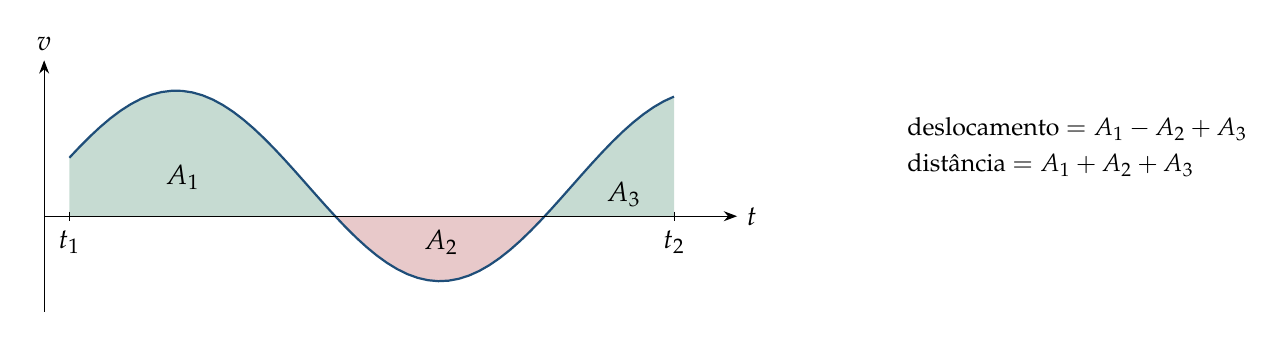
\begin{tikzpicture}[xscale=1.6, yscale=1.1, >=Stealth]
  \def\v#1{(1.1*sin(1.5*#1 r) + 0.35)}
  \fill[verde!25, domain=0.2:2.31, samples=30] plot (\x,{\v{\x}}) -- (2.31,0) -- (0.2,0) -- cycle;
  \fill[vermelho!25, domain=2.31:3.973, samples=30] plot (\x,{\v{\x}}) -- (3.973,0) -- (2.31,0) -- cycle;
  \fill[verde!25, domain=3.973:5.0, samples=30] plot (\x,{\v{\x}}) -- (5.0,0) -- (3.973,0) -- cycle;
  \draw[thick, azul, domain=0.2:5.0, samples=60] plot (\x,{\v{\x}});
  \draw[->] (0,0) -- (5.5,0) node[right] {$t$};
  \draw[->] (0,-1.1) -- (0,1.8) node[above] {$v$};
  \node at (1.1,0.45) {$A_1$}; \node at (3.15,-0.3) {$A_2$}; \node at (4.6,0.25) {$A_3$};
  \draw (0.2,0.05)--(0.2,-0.05) node[below] {$t_1$};
  \draw (5.0,0.05)--(5.0,-0.05) node[below] {$t_2$};
  \node[font=\small, align=left] at (8.2,0.8) {deslocamento $=A_1-A_2+A_3$\\[2pt] distância $=A_1+A_2+A_3$};
\end{tikzpicture}
\end{center}
\end{definicao}

\begin{exemplo}[{Exemplo 4.6 --- da aceleração à distância (questão 5.4.72)}]
$a(t)=2t+3$ (m/s$^2$), $v(0)=-4$ m/s, $0\le t\le3$. Encontre (a) $v(t)$ e (b) a distância percorrida.

\textbf{(a)} $v(t)=\displaystyle\int(2t+3)\dt=t^2+3t+C$; $v(0)=C=-4$ \;$\Rightarrow$\; $v(t)=t^2+3t-4=(t+4)(t-1)$.

\textbf{(b) Sinal de $v$:} $v<0$ em $[0,1)$ (partícula indo para a esquerda) e $v>0$ em $(1,3]$. Primitiva de $v$: $s(t)=\dfrac{t^3}{3}+\dfrac{3t^2}{2}-4t$ (posição com $s(0)=0$).
\[
\int_0^1 v\dt=s(1)-s(0)=\frac13+\frac32-4=\frac{2+9-24}{6}=-\frac{13}{6},
\]
\[
\int_1^3 v\dt=s(3)-s(1)=\Big(9+\frac{27}{2}-12\Big)-\Big(-\frac{13}{6}\Big)=\frac{21}{2}+\frac{13}{6}=\frac{63+13}{6}=\frac{38}{3}.
\]
\[
\text{distância}=\int_0^3|v|\dt=\frac{13}{6}+\frac{38}{3}=\frac{13+76}{6}=\frac{89}{6}\approx14{,}83\ \text{m}.
\]
\textbf{Comparando com o deslocamento:} $\displaystyle\int_0^3 v\dt=-\frac{13}{6}+\frac{38}{3}=\frac{63}{6}=\frac{21}{2}=10{,}5$ m. A partícula anda $2{,}17$ m para a esquerda, para em $t=1$, e anda $12{,}67$ m para a direita: termina $10{,}5$ m à direita de onde começou, tendo percorrido $14{,}83$ m.

\textbf{Verificação:} $s'(t)=t^2+3t-4=v(t)$ \ok; $v'(t)=2t+3=a(t)$ \ok.
\end{exemplo}

\begin{exemplo}[{Exemplo 4.7 --- vazão e densidade (questões 5.4.74 e 5.4.73)}]
\textbf{(a)} Água escoa de um tanque a $r(t)=200-4t$ L/min, $0\le t\le50$. Quanto escoa nos primeiros 10 minutos?
\[
\int_0^{10}(200-4t)\dt=\Big[200t-2t^2\Big]_0^{10}=2000-200=1800\ \text{L}.
\]
Geometria: $r$ é uma reta de $200$ a $160$ em $[0,10]$: trapézio $\frac{200+160}{2}\cdot10=1800$ \ok.

\textbf{(b)} Barra de 4 m com densidade $\rho(x)=9+2\sqrt x$ kg/m. Massa total:
\[
\int_0^4\big(9+2x^{1/2}\big)\dx=\Big[9x+2\cdot\frac{x^{3/2}}{3/2}\Big]_0^4=\Big[9x+\frac43x^{3/2}\Big]_0^4=36+\frac43\cdot8=36+\frac{32}{3}=\frac{140}{3}\approx46{,}7\ \text{kg}.
\]
Unidade: (kg/m)$\cdot$m $=$ kg \ok. Ordem de grandeza: $\rho$ vai de $9$ a $13$, largura $4$ $\Rightarrow$ entre $36$ e $52$ \ok.
\end{exemplo}

\begin{exercicios}[{Exercícios similares --- Parte 4}]
\begin{enumerate}[leftmargin=1.6em, itemsep=2pt, label=\textbf{4.\arabic*}]
\item Derive: (a) $g(x)=\displaystyle\int_0^x\sqrt{t+t^3}\dt$; \;(b) $h(x)=\displaystyle\int_1^{e^x}\ln t\dt$; \;(c) $y=\displaystyle\int_{\cos x}^{\sen x}\frac{1}{1+t^2}\dt$.
\item Encontre $f$ e $a$ tais que $\displaystyle 3+\int_a^x f(t)\dt=x^3$ para todo $x$.
\item Calcule e interprete como área ou diferença de áreas: $\displaystyle\int_0^2(2x-x^3)\dx$.
\item Calcule $\displaystyle\int_{-2}^{2}f(x)\dx$ para $f(x)=\begin{cases}2,&-2\le x\le0\\4-x^2,&0<x\le2\end{cases}$
\item $v(t)=t^2-2t-3$ m/s em $[2,4]$: deslocamento e distância (5.4.70).
\item $v(t)=3t-5$ m/s em $[0,3]$: deslocamento e distância (5.4.69).
\item $a(t)=t+4$, $v(0)=5$, $0\le t\le10$: $v(t)$ e distância (5.4.71). Por que aqui distância $=$ deslocamento?
\item Se $r(t)$ (L/min) é a taxa com que água \emph{entra} em um tanque que tem $25\,000$ L em $t=0$, o que representa $25\,000+\displaystyle\int_0^{4}r(t)\dt$? E se $r$ ficar negativa em parte do intervalo?
\item O que está errado em $\displaystyle\int_{-2}^{1}\frac{1}{x^4}\dx=\Big[-\frac{1}{3x^3}\Big]_{-2}^{1}=-\frac13-\frac{1}{24}=-\frac{3}{8}$?
\end{enumerate}
\end{exercicios}

\section[Regra da Substituição (5.5)]{A Regra da Substituição (5.5) --- a regra da cadeia lida ao contrário}

\begin{definicao}[{Regra da Substituição}]
Se $u=g(x)$ é derivável e $f$ é contínua na imagem de $g$:
\[
\int f\big(g(x)\big)\,g'(x)\dx=\int f(u)\du,\qquad du=g'(x)\dx .
\]
Para integrais definidas, \textbf{troque também os limites}:
\[
\int_a^b f\big(g(x)\big)\,g'(x)\dx=\int_{g(a)}^{g(b)}f(u)\du .
\]
Por que funciona: se $F'=f$, então $\frac{d}{dx}F(g(x))=F'(g(x))g'(x)=f(g(x))g'(x)$ (regra da cadeia). A substituição só ``desfaz'' a cadeia. O $du=g'(x)\dx$ vem da notação de Leibniz: $\frac{du}{dx}=g'(x)$.
\end{definicao}

\begin{metodo}[{Como reconhecer e como executar}]
\textbf{Reconhecer:} há uma função ``de dentro'' $g(x)$ --- argumento de $\sen$, $\cos$, $e^{(\cdot)}$, $\ln$; base de uma potência; radicando; denominador --- \emph{e} a derivada $g'(x)$ aparece multiplicando, a menos de uma constante.

\textbf{Executar:}
\begin{enumerate}[leftmargin=1.6em, itemsep=1pt]
\item $u=g(x)$ (a função de dentro).
\item $du=g'(x)\dx$. Se falta só uma constante $k$, escreva $g'(x)\dx=du$ e ajuste: $\dx=\frac{du}{g'(x)}$.
\item Reescreva a integral \textbf{inteiramente} em $u$. \emph{Nenhum $x$ pode sobrar.} Se sobrar, a substituição está errada ou não é o método.
\item Integre em $u$ (tabela).
\item Indefinida: volte para $x$ e $+C$. Definida: use os limites novos $g(a)$, $g(b)$ e \emph{não} volte para $x$.
\item Verifique derivando (indefinida) ou pelo sinal/tamanho esperado (definida).
\end{enumerate}
\textbf{Não é substituição simples} quando o fator que sobra não é constante: $\int e^{x^2}\dx$ (falta um $x$), $\int x^2\cos(x^4)\dx$ (falta $x^3$, sobra $x^2$). Essas não têm primitiva elementar --- não invente uma.
\end{metodo}

\begin{exemplo}[{Exemplo 5.1 --- o exemplo-modelo (Stewart, 5.5, Exemplo 1)}]
$\displaystyle\int x^3\cos(x^4+2)\dx$.

\textbf{Classificação:} $\cos(\;\cdot\;)$ com argumento $x^4+2$, e a derivada $4x^3$ aparece a menos da constante $4$. Substituição.

$u=x^4+2$, \; $du=4x^3\dx$ \;$\Rightarrow$\; $x^3\dx=\dfrac{du}{4}$.
\[
\int x^3\cos(x^4+2)\dx=\int\cos u\cdot\frac{du}{4}=\frac14\int\cos u\du=\frac14\sen u+C=\frac14\sen(x^4+2)+C .
\]
\textbf{Verificação:} $\dfrac{d}{dx}\Big[\tfrac14\sen(x^4+2)\Big]=\tfrac14\cos(x^4+2)\cdot4x^3=x^3\cos(x^4+2)$ \ok.
\end{exemplo}

\begin{exemplo}[{Exemplo 5.2 --- raiz de função afim}]
$\displaystyle\int\sqrt{2x+1}\dx$. \quad $u=2x+1$, $du=2\dx$, $\dx=\dfrac{du}{2}$:
\[
\int u^{1/2}\frac{du}{2}=\frac12\cdot\frac{u^{3/2}}{3/2}+C=\frac13u^{3/2}+C=\frac13(2x+1)^{3/2}+C .
\]
Verificação: $\frac13\cdot\frac32(2x+1)^{1/2}\cdot2=(2x+1)^{1/2}$ \ok.
\end{exemplo}

\begin{exemplo}[{Exemplo 5.3 --- o $x$ do numerador é a pista}]
$\displaystyle\int\frac{x}{\sqrt{1-4x^2}}\dx$. \quad $u=1-4x^2$, $du=-8x\dx$ \;$\Rightarrow$\; $x\dx=-\dfrac{du}{8}$:
\[
\int u^{-1/2}\Big(-\frac{du}{8}\Big)=-\frac18\cdot\frac{u^{1/2}}{1/2}+C=-\frac14\sqrt u+C=-\frac14\sqrt{1-4x^2}+C .
\]
(Sem o $x$ no numerador seria $\arcsen(2x)/2$ --- outra integral, outra técnica. O fator $x$ decide.)
\end{exemplo}

\begin{exemplo}[{Exemplo 5.4 --- $\int\tg x\dx$ e o padrão $\int\frac{g'}{g}$}]
$\displaystyle\int\tg x\dx=\int\frac{\sen x}{\cos x}\dx$. \quad $u=\cos x$, $du=-\sen x\dx$:
\[
\int\frac{-du}{u}=-\ln|u|+C=-\ln|\cos x|+C=\ln|\sec x|+C .
\]
Padrão geral: $\displaystyle\int\frac{g'(x)}{g(x)}\dx=\ln|g(x)|+C$. Exemplos: $\int\frac{2x}{x^2+1}\dx=\ln(x^2+1)+C$; $\int\frac{e^x}{e^x+3}\dx=\ln(e^x+3)+C$.
\end{exemplo}

\begin{exemplo}[{Exemplo 5.5 --- definida, trocando os limites (Stewart, 5.5, Exemplo 7)}]
$\displaystyle\int_1^2\frac{dx}{(3-5x)^2}$. \quad $u=3-5x$, $du=-5\dx$, $\dx=-\dfrac{du}{5}$. Limites: $x=1\Rightarrow u=-2$; $x=2\Rightarrow u=-7$.
\begin{align*}
\int_1^2\frac{dx}{(3-5x)^2}&=-\frac15\int_{-2}^{-7}u^{-2}\du=-\frac15\Big[-\frac1u\Big]_{-2}^{-7}
=-\frac15\Big[\Big(-\frac{1}{-7}\Big)-\Big(-\frac{1}{-2}\Big)\Big]\\
&=-\frac15\Big[\frac17-\frac12\Big]=-\frac15\cdot\Big(-\frac{5}{14}\Big)=\frac{1}{14}.
\end{align*}
\textbf{Conferindo:} em $[1,2]$ o integrando é positivo e vai de $\frac14$ a $\frac1{49}$, então a integral está entre $\frac1{49}\approx0{,}02$ e $\frac14$: $\frac1{14}\approx0{,}071$ \ok. Note que os limites em $u$ ficaram ``ao contrário'' ($-2$ para $-7$) --- isso é normal; não os reordene.
\end{exemplo}

\begin{exemplo}[{Exemplo 5.6 --- $\ln$ como função de dentro}]
$\displaystyle\int_1^{e}\frac{\ln x}{x}\dx$. \quad $u=\ln x$, $du=\dfrac{dx}{x}$; $x=1\Rightarrow u=0$; $x=e\Rightarrow u=1$:
\[
\int_0^1 u\du=\Big[\frac{u^2}{2}\Big]_0^1=\frac12 .
\]
\end{exemplo}

\begin{definicao}[{Simetria (Teorema 7 da seção 5.5) --- economiza conta e evita erro}]
Se $f$ é contínua em $[-a,a]$:
\[
f\ \text{par}\ (f(-x)=f(x))\ \Rightarrow\ \int_{-a}^{a}f\dx=2\int_0^a f\dx;
\qquad
f\ \text{ímpar}\ (f(-x)=-f(x))\ \Rightarrow\ \int_{-a}^{a}f\dx=0 .
\]
Geometria: função par tem gráfico simétrico ao eixo $y$ (duas áreas iguais); ímpar tem simetria pela origem (as áreas se cancelam). Regras rápidas: par $\times$ par $=$ par; ímpar $\times$ ímpar $=$ par; par $\times$ ímpar $=$ ímpar; $x^{\text{par}}$, $\cos$, $|x|$ são pares; $x^{\text{ímpar}}$, $\sen$, $\tg$ são ímpares.
\end{definicao}

\begin{exemplo}[{Exemplo 5.7 --- simetria (Stewart, 5.5, Exemplos 9 e 10)}]
\textbf{(a)} $\displaystyle\int_{-2}^{2}(x^6+1)\dx=2\int_0^2(x^6+1)\dx=2\Big[\frac{x^7}{7}+x\Big]_0^2=2\Big(\frac{128}{7}+2\Big)=\frac{284}{7}$.

\textbf{(b)} $\displaystyle\int_{-1}^{1}\frac{\tg x}{1+x^2+x^4}\dx=0$: numerador ímpar, denominador par, quociente ímpar. Sem calcular nada.
\end{exemplo}

\begin{armadilha}[{Onde a substituição dá errado}]
\begin{itemize}[leftmargin=1.4em, itemsep=1pt]
\item Sobrar $x$ na integral em $u$ (ex.: escrever $\int x\cos u\du$). Ou você resolve o $x$ em função de $u$, ou o método não é este.
\item Esquecer o fator de ajuste: $\int\cos(5x)\dx=\frac15\sen(5x)+C$, não $\sen(5x)+C$. (Derive e veja o $5$ aparecer.)
\item Na definida, misturar: voltar para $x$ \emph{e} usar os limites em $u$, ou ficar em $u$ e usar os limites em $x$. Escolha um caminho.
\item Escolher $u$ = ``a expressão toda'' em vez da função de dentro. Em $\int x^3\cos(x^4+2)\dx$, $u$ é $x^4+2$, não $\cos(x^4+2)$.
\item Esquecer o módulo em $\ln|u|$ quando $u$ pode ser negativo.
\end{itemize}
\end{armadilha}

\begin{exercicios}[{Exercícios similares --- Parte 5}]
\begin{enumerate}[leftmargin=1.6em, itemsep=2pt, label=\textbf{5.\arabic*}]
\item $\displaystyle\int x^2e^{x^3}\dx$
\item $\displaystyle\int\frac{(\ln x)^2}{x}\dx$
\item $\displaystyle\int x\sqrt{x^2+1}\dx$
\item $\displaystyle\int_0^1 xe^{x^2}\dx$
\item $\displaystyle\int_0^{\pi/2}\cos x\,\sen(\sen x)\dx$
\item $\displaystyle\int_0^{\sqrt\pi}x\cos(x^2)\dx$ --- interprete o resultado.
\item $\displaystyle\int_{-\pi/4}^{\pi/4}\big(x^3+x^4\tg x\big)\dx$
\item $\displaystyle\int\frac{\sec^2x}{1+\tg x}\dx$
\end{enumerate}
\end{exercicios}

\section[Aplicações (6.1--6.3)]{Aplicações (6.1--6.3): toda fórmula é uma soma de Riemann}

O capítulo 6 não tem técnica nova. Cada fórmula nasce do mesmo procedimento da Parte 3: \textbf{fatiar} a região ou o sólido em $n$ pedaços de largura $\Delta x$, aproximar cada pedaço por uma figura simples, \textbf{somar} e passar ao \textbf{limite}. Se você souber montar a soma de Riemann, a fórmula sai sozinha --- e é isso que a professora pede em 7.3/7.4 (``fazer a modelagem e escrever a soma de Riemann associada'').

\subsection{Área entre curvas (6.1)}

\begin{definicao}[{Área entre $y=f(x)$ (em cima) e $y=g(x)$ (embaixo), $a\le x\le b$}]
Fatia $i$: retângulo de base $\Delta x$ e altura $f(x_i^*)-g(x_i^*)$ (topo menos base).
\[
A=\lim_{n\to\infty}\sum_{i=1}^n\big[f(x_i^*)-g(x_i^*)\big]\Delta x=\int_a^b\big[f(x)-g(x)\big]\dx .
\]
Se as curvas se cruzam dentro do intervalo, separe nos cruzamentos: $A=\int_a^b|f(x)-g(x)|\dx$. Se a região é mais fácil de descrever em $y$: $A=\displaystyle\int_c^d\big[x_{\text{dir}}(y)-x_{\text{esq}}(y)\big]\,dy$ (direita menos esquerda).
\end{definicao}

\begin{metodo}[{Roteiro}]
(1) Esboce. (2) Interseções: resolva $f(x)=g(x)$. (3) Quem está em cima? Teste um ponto entre as interseções. (4) Se trocam de posição, separe. (5) Integre. (6) Área tem que dar positiva.
\end{metodo}

\begin{exemplo}[{Exemplo 6.1 --- parábola e reta}]
Área entre $y=x^2$ e $y=x+2$.

\textbf{Interseções:} $x^2=x+2\Rightarrow x^2-x-2=0\Rightarrow(x-2)(x+1)=0\Rightarrow x=-1,\ 2$.

\textbf{Quem está em cima:} em $x=0$, reta $=2>0=$ parábola. Topo: $x+2$; base: $x^2$.
\begin{align*}
A=\int_{-1}^{2}\big[(x+2)-x^2\big]\dx&=\Big[\frac{x^2}{2}+2x-\frac{x^3}{3}\Big]_{-1}^{2}
=\Big(2+4-\frac83\Big)-\Big(\frac12-2+\frac13\Big)\\
&=\frac{10}{3}-\Big(-\frac76\Big)=\frac{20}{6}+\frac76=\frac{27}{6}=\frac92 .
\end{align*}
\textbf{Soma de Riemann associada:} $\displaystyle\lim_{n\to\infty}\sum_{i=1}^n\big[(x_i+2)-x_i^2\big]\Delta x$ com $\Delta x=\frac3n$, $x_i=-1+\frac{3i}{n}$.
\end{exemplo}

\begin{exemplo}[{Exemplo 6.2 --- curvas que se cruzam}]
Área entre $y=\sen x$ e $y=\cos x$ de $x=0$ a $x=\pi/2$. Cruzam em $\tg x=1\Rightarrow x=\pi/4$. Em $[0,\pi/4]$ o cosseno está em cima; em $[\pi/4,\pi/2]$ o seno.
\begin{align*}
A&=\int_0^{\pi/4}(\cos x-\sen x)\dx+\int_{\pi/4}^{\pi/2}(\sen x-\cos x)\dx\\
&=\Big[\sen x+\cos x\Big]_0^{\pi/4}+\Big[-\cos x-\sen x\Big]_{\pi/4}^{\pi/2}\\
&=\Big(\frac{\sqrt2}{2}+\frac{\sqrt2}{2}-0-1\Big)+\Big(-0-1+\frac{\sqrt2}{2}+\frac{\sqrt2}{2}\Big)\\
&=(\sqrt2-1)+(\sqrt2-1)=2\sqrt2-2 .
\end{align*}
Se você integrasse $\cos x-\sen x$ direto em $[0,\pi/2]$ daria $0$ --- a área ``negativa'' cancelaria a positiva. Separar nos cruzamentos não é opcional.
\end{exemplo}

\subsection{Volumes por fatiamento: discos e anéis (6.2)}

\begin{definicao}[{Volume por seções transversais}]
Se a seção transversal do sólido em $x$ tem área $A(x)$, a fatia $i$ é um ``cilindro'' fino de base $A(x_i^*)$ e espessura $\Delta x$:
\[
V=\lim_{n\to\infty}\sum_{i=1}^n A(x_i^*)\Delta x=\int_a^b A(x)\dx .
\]
\textbf{Disco} (girar a região sob $y=f(x)$ em torno do eixo $x$): $A(x)=\pi\big[f(x)\big]^2$.

\textbf{Anel} (região entre $f$ em cima e $g$ embaixo, eixo $x$): $A(x)=\pi\big([f(x)]^2-[g(x)]^2\big)=\pi(R^2-r^2)$.

\textbf{Eixo deslocado} $y=k$: raios medidos até a reta, $R=|f(x)-k|$, $r=|g(x)-k|$. Girar em torno do eixo $y$ com região descrita em $y$: $V=\int_c^d\pi[x(y)]^2\,dy$.
\end{definicao}

\begin{exemplo}[{Exemplo 6.3 --- disco}]
Região sob $y=\sqrt x$, $0\le x\le4$, girada em torno do eixo $x$.
\[
V=\int_0^4\pi\big(\sqrt x\big)^2\dx=\pi\int_0^4x\dx=\pi\Big[\frac{x^2}{2}\Big]_0^4=8\pi .
\]
Cada fatia é um disco de raio $\sqrt{x_i^*}$ e espessura $\Delta x$: volume $\pi(\sqrt{x_i^*})^2\Delta x$.
\end{exemplo}

\begin{exemplo}[{Exemplo 6.4 --- anel, eixo $x$ e eixo deslocado}]
Região entre $y=x$ e $y=x^2$ ($0\le x\le1$; em cima está $y=x$).

\textbf{(a) Em torno do eixo $x$:} $R=x$, $r=x^2$:
\[
V=\pi\int_0^1\big(x^2-x^4\big)\dx=\pi\Big[\frac{x^3}{3}-\frac{x^5}{5}\Big]_0^1=\pi\Big(\frac13-\frac15\Big)=\frac{2\pi}{15}.
\]
\textbf{(b) Em torno de $y=2$:} agora o raio externo é a distância da curva \emph{de baixo} até $y=2$: $R=2-x^2$, $r=2-x$.
\begin{align*}
V&=\pi\int_0^1\big[(2-x^2)^2-(2-x)^2\big]\dx=\pi\int_0^1\big[(4-4x^2+x^4)-(4-4x+x^2)\big]\dx\\
&=\pi\int_0^1\big(x^4-5x^2+4x\big)\dx
=\pi\Big[\frac{x^5}{5}-\frac{5x^3}{3}+2x^2\Big]_0^1=\pi\Big(\frac15-\frac53+2\Big)=\pi\cdot\frac{3-25+30}{15}=\frac{8\pi}{15}.
\end{align*}
Erro comum: usar $R=x$, $r=x^2$ em (b). O raio é sempre a distância até o \emph{eixo de rotação}, não até o eixo $x$.
\end{exemplo}

\subsection{Cascas cilíndricas (6.3)}

\begin{definicao}[{Volume por cascas --- girar em torno do eixo $y$ a região sob $y=f(x)$, $0\le a\le x\le b$}]
Fatia $i$: ao girar o retângulo de base $\Delta x$ e altura $f(x_i^*)$ em torno do eixo $y$, obtém-se uma casca cilíndrica de raio $x_i^*$, altura $f(x_i^*)$ e espessura $\Delta x$. ``Desenrolada'', é uma placa de comprimento $2\pi x_i^*$ (circunferência), altura $f(x_i^*)$ e espessura $\Delta x$:
\[
V=\lim_{n\to\infty}\sum_{i=1}^n 2\pi x_i^*\,f(x_i^*)\,\Delta x=\int_a^b 2\pi x\,f(x)\dx .
\]
Região entre $f$ (cima) e $g$ (baixo): altura $f(x)-g(x)$. Eixo $x=k$: raio $|x-k|$.

\textbf{Quando usar:} rotação em torno do eixo $y$ (ou de uma reta vertical) com a região dada por $y=f(x)$ --- cascas evitam isolar $x$ em função de $y$. Rotação em torno do eixo $x$ com $y=f(x)$: discos/anéis. Regra prática: fatias \emph{perpendiculares} ao eixo de rotação $\to$ discos/anéis; fatias \emph{paralelas} $\to$ cascas.
\end{definicao}

\begin{exemplo}[{Exemplo 6.5 --- o exemplo clássico das cascas (Stewart, 6.3, Exemplo 1)}]
Região sob $y=2x^2-x^3$ (de $x=0$ a $x=2$, onde $y=0$) girada em torno do eixo $y$. Isolar $x$ em função de $y$ aqui seria inviável $\Rightarrow$ cascas.
\begin{align*}
V&=\int_0^2 2\pi x\big(2x^2-x^3\big)\dx=2\pi\int_0^2\big(2x^3-x^4\big)\dx\\
&=2\pi\Big[\frac{x^4}{2}-\frac{x^5}{5}\Big]_0^2=2\pi\Big(8-\frac{32}{5}\Big)=2\pi\cdot\frac85=\frac{16\pi}{5}.
\end{align*}
\end{exemplo}

\begin{exemplo}[{Exemplo 6.6 --- os dois métodos dão o mesmo volume}]
Região sob $y=x^2$, $0\le x\le1$, girada em torno do eixo $y$.

\textbf{Cascas:} $V=\displaystyle\int_0^1 2\pi x\cdot x^2\dx=2\pi\Big[\frac{x^4}{4}\Big]_0^1=\frac{\pi}{2}$.

\textbf{Anéis (fatiando em $y$):} em altura $y$, o anel vai de $x=\sqrt y$ (curva) até $x=1$ (borda): $R=1$, $r=\sqrt y$.
$V=\displaystyle\int_0^1\pi\big(1^2-(\sqrt y)^2\big)\,dy=\pi\int_0^1(1-y)\,dy=\pi\Big[y-\frac{y^2}{2}\Big]_0^1=\frac{\pi}{2}$ \ok.
\end{exemplo}

\begin{armadilha}[{Capítulo 6}]
\begin{itemize}[leftmargin=1.4em, itemsep=1pt]
\item Área entre curvas: integrar $f-g$ sem checar quem está em cima; não separar nos cruzamentos.
\item Volumes: elevar ao quadrado \emph{antes} de subtrair ($\pi(R-r)^2$ é errado; é $\pi(R^2-r^2)$).
\item Eixo deslocado: raio $=$ distância até o eixo de rotação.
\item Cascas: esquecer o fator $2\pi x$ (o raio da casca) ou usar $x$ quando o eixo é $x=k$.
\item Sempre esboce a região e uma fatia típica: a fórmula deve ser \emph{lida} do desenho, não lembrada.
\end{itemize}
\end{armadilha}

\begin{exercicios}[{Exercícios similares --- Parte 6}]
\begin{enumerate}[leftmargin=1.6em, itemsep=2pt, label=\textbf{6.\arabic*}]
\item Área entre $y=x^2$ e $y=2x$.
\item Área entre $y=x^3$ e $y=x$ (use simetria).
\item Área da região limitada por $x=2y-y^2$ e o eixo $y$ (integre em $y$).
\item Volume: região sob $y=1/x$, $1\le x\le2$, girada em torno do eixo $x$.
\item Volume: região entre $y=x$ e $y=x^2$ girada em torno do eixo $y$ (cascas).
\item Volume: região sob $y=\sqrt x$, $0\le x\le4$, girada em torno do eixo $y$ --- por cascas e por anéis.
\end{enumerate}
\end{exercicios}

\newpage
\section{Checklist de armadilhas e formulário de bolso}

\begin{armadilha}[{Os 16 erros que mais custam ponto na P1 --- confira antes de entregar}]
\begin{multicols}{2}
\begin{enumerate}[leftmargin=1.5em, itemsep=1pt]
\item Faltou $+C$ na indefinida (ou sobrou $C$ na definida).
\item $\int\sen=-\cos$; $\int\cos=\sen$. Derive para conferir o sinal.
\item Radianos. $\cos0=1$, $\sen\frac\pi2=1$, $\cos\pi=-1$.
\item $\int x^{-1}\dx=\ln|x|+C$, não $x^0/0$.
\item Não dividiu termo a termo / não expandiu antes de integrar.
\item Descartou primitiva em forma fatorada sem derivá-la.
\item Na substituição, sobrou $x$ na integral em $u$.
\item Na definida com substituição, não trocou os limites (ou misturou $x$ e $u$).
\item Aplicou TFC2 com integrando descontínuo no intervalo.
\item $F(a)-F(b)$ em vez de $F(b)-F(a)$.
\item Chamou a integral de ``área'' quando $f$ muda de sinal.
\item Confundiu distância com deslocamento (esqueceu $|v|$ e os zeros de $v$).
\item Dentro do $\sum$, tratou $n$ como variável ou esqueceu o $\Delta x$.
\item $x_i=a+i\Delta x$: esqueceu o $a$.
\item $\frac{d}{dx}\int_a^b f=0$; $\frac{d}{dx}\int_a^x f(t)\dt=f(x)$; com $u(x)$ em cima, multiplica por $u'$.
\item ``Duas primitivas diferem por constante'' só vale em um \emph{intervalo}.
\end{enumerate}
\end{multicols}
\end{armadilha}

\newpage
\begin{definicao}[{Formulário --- tudo da P1 em uma página}]
\small
\textbf{Soma de Riemann e integral definida}
\[
\int_a^b f(x)\dx=\lim_{n\to\infty}\sum_{i=1}^n f(x_i^*)\Delta x,\qquad \Delta x=\frac{b-a}{n},\qquad x_i=a+i\Delta x,\qquad \bar x_i=a+\big(i-\tfrac12\big)\Delta x
\]
\[
L_n=\sum_{i=1}^n f(x_{i-1})\Delta x,\qquad R_n=\sum_{i=1}^n f(x_i)\Delta x,\qquad M_n=\sum_{i=1}^n f(\bar x_i)\Delta x;\qquad f\ \text{crescente}\ \Rightarrow\ L_n\le\int_a^b f\le R_n
\]
\[
\sum_{i=1}^n i=\frac{n(n+1)}{2},\qquad \sum_{i=1}^n i^2=\frac{n(n+1)(2n+1)}{6},\qquad \sum_{i=1}^n i^3=\Big[\frac{n(n+1)}{2}\Big]^2,\qquad \sum_{i=1}^n c=nc
\]
\textbf{Propriedades:} $\int_a^a f=0$; \ $\int_b^a f=-\int_a^b f$; \ $\int_a^b c\dx=c(b-a)$; \ linearidade; \ $\int_a^c f+\int_c^b f=\int_a^b f$; \ $f\ge g\Rightarrow\int_a^b f\ge\int_a^b g$; \ $m\le f\le M\Rightarrow m(b-a)\le\int_a^b f\le M(b-a)$.

\textbf{TFC} \ ($f$ contínua, $F'=f$)
\[
\frac{d}{dx}\int_a^x f(t)\dt=f(x),\qquad
\frac{d}{dx}\int_{u(x)}^{v(x)}f(t)\dt=f\big(v(x)\big)v'(x)-f\big(u(x)\big)u'(x),\qquad
\int_a^b f(x)\dx=F(b)-F(a)
\]
\textbf{Variação total / cinemática}
\[
\int_a^b F'(x)\dx=F(b)-F(a),\qquad
\text{desloc.}=\int_{t_1}^{t_2}v\dt,\qquad
\text{dist.}=\int_{t_1}^{t_2}|v|\dt,\qquad
\int_{t_1}^{t_2}a\dt=v(t_2)-v(t_1)
\]
\textbf{Tabela} (todas com $+C$)
\[
\int x^n\dx=\frac{x^{n+1}}{n+1}\ (n\ne-1),\qquad
\int\frac{dx}{x}=\ln|x|,\qquad
\int e^x\dx=e^x,\qquad
\int a^x\dx=\frac{a^x}{\ln a}
\]
\[
\int\sen x\dx=-\cos x,\qquad
\int\cos x\dx=\sen x,\qquad
\int\senh x\dx=\cosh x,\qquad
\int\cosh x\dx=\senh x
\]
\[
\int\sec^2x\dx=\tg x,\qquad
\int\cossec^2x\dx=-\cotg x,\qquad
\int\frac{dx}{1+x^2}=\arctg x
\]
\[
\int\sec x\tg x\dx=\sec x,\qquad
\int\cossec x\cotg x\dx=-\cossec x,\qquad
\int\frac{dx}{\sqrt{1-x^2}}=\arcsen x
\]
\textbf{Substituição} \ ($u=g(x)$, $du=g'(x)\dx$)
\[
\int f\big(g(x)\big)g'(x)\dx=\int f(u)\du,\qquad
\int_a^b f\big(g(x)\big)g'(x)\dx=\int_{g(a)}^{g(b)}f(u)\du,\qquad
\int\frac{g'(x)}{g(x)}\dx=\ln|g(x)|+C
\]
\textbf{Simetria:} $f$ par $\Rightarrow\int_{-a}^a f=2\int_0^a f$; \ $f$ ímpar $\Rightarrow\int_{-a}^a f=0$.

\textbf{Aplicações}
\[
A=\int_a^b\big[f(x)-g(x)\big]\dx\ \ \text{(cima $-$ baixo)},\qquad
A=\int_c^d\big[x_{\text{dir}}(y)-x_{\text{esq}}(y)\big]\,dy
\]
\[
V=\int_a^b A(x)\dx;\qquad \text{disco: }A=\pi[f(x)]^2;\qquad \text{anel: }A=\pi\big(R^2-r^2\big)
\]
\[
\text{cascas (eixo $y$): }V=\int_a^b 2\pi x\,f(x)\dx\qquad(\text{raio }x,\ \text{altura }f(x),\ \text{espessura }dx)
\]
\textbf{Identidades:} $\tg^2x=\sec^2x-1$; \ $\sen^2x=\frac{1-\cos2x}{2}$; \ $\cos^2x=\frac{1+\cos2x}{2}$; \ $\sen x\cos x=\frac12\sen2x$; \ $\sen^2x+\cos^2x=1$.
\end{definicao}

\section{Gabarito dos exercícios similares}

\subsection*{Parte 1}
\begin{description}[leftmargin=2.2em, itemsep=2pt, font=\bfseries]
\item[1.1] (a) Falso: $f(x)=x$ tem $f'=1>0$ mas $f<0$ para $x<0$. (b) Verdadeiro: $(f-g)'=0$, logo $f'=g'$. (c) Falso: $|x|$ é contínua em $0$ e não derivável em $0$.
\item[1.2] No instante $t=3$ min o volume está \emph{diminuindo} à taxa de $12$ L/min (sai mais água do que entra). Unidade: L/min.
\item[1.3] (a) $[x\sen x]_0^{\pi}=\pi\sen\pi-0=0$. \ (b) $0$ (derivada de uma constante). \ (c) $x\sen x$.
\item[1.4] Positiva: $\ln x>0$ em $(1,2]$, então a integral é a área sob uma curva positiva (propriedade 6).
\end{description}

\subsection*{Parte 2}
\begin{description}[leftmargin=2.2em, itemsep=2pt, font=\bfseries]
\item[2.1] $\dfrac{x^3-2x}{x^2}=x-\dfrac2x$ \;$\Rightarrow$\; $\dfrac{x^2}{2}-2\ln|x|+C$.
\item[2.2] $u^2-u-6$ \;$\Rightarrow$\; $\dfrac{u^3}{3}-\dfrac{u^2}{2}-6u+C$.
\item[2.3] $\sec^2\theta+1$ \;$\Rightarrow$\; $\tg\theta+\theta+C$.
\item[2.4] $f'(x)=2x+6x^2-4x^3+12$; \; $f(x)=-x^4+2x^3+x^2+12x+4$.
\item[2.5] $f(x)=x^2+x+C$; $f'(1)=3$; tangente $y=3(x-1)+2+C$ passa pela origem $\Rightarrow C=1$. \; $f(x)=x^2+x+1$.
\item[2.6] $v=-10\cos t+3\sen t+C_1$; $s=-10\sen t-3\cos t+C_1t+C_2$; $s(0)=0\Rightarrow C_2=3$; $s(2\pi)=2\pi C_1=12\Rightarrow C_1=6/\pi$. \; $s(t)=-10\sen t-3\cos t+\dfrac{6}{\pi}t+3$.
\end{description}

\subsection*{Parte 3}
\begin{description}[leftmargin=2.2em, itemsep=2pt, font=\bfseries]
\item[3.1] $\Delta x=\tfrac12$. $R_4=\tfrac12\big[\tfrac18+1+\tfrac{27}{8}+8\big]=6{,}25$ (super); $L_4=\tfrac12\big[0+\tfrac18+1+\tfrac{27}{8}\big]=2{,}25$ (sub). $x^3$ é crescente em $[0,2]$; exato $4$.
\item[3.2] $R_4=\tfrac14\big[\tfrac1{1{,}25}+\tfrac1{1{,}5}+\tfrac1{1{,}75}+\tfrac12\big]\approx0{,}6345$ (sub: $1/x$ é decrescente); $L_4\approx0{,}7595$ (super); exato $\ln2\approx0{,}6931$.
\item[3.3] $\Delta x=\tfrac2n$, $x_i=1+\tfrac{2i}{n}$, $f(x_i)=2+\tfrac{4i}{n}+\tfrac{4i^2}{n^2}$; $R_n=4+4\tfrac{n+1}{n}+\tfrac43\tfrac{(n+1)(2n+1)}{n^2}\to4+4+\tfrac83=\tfrac{32}{3}$. TFC: $[x^3/3+x]_1^3=12-\tfrac43=\tfrac{32}3$ \ok.
\item[3.4] (a) $\displaystyle\int_2^7(5x^3-4x)\dx$. \ (b) $\Delta x=\tfrac3n$, $x_i=\tfrac{3i}{n}$, $[0,3]$: $\displaystyle\int_0^3\sqrt{1+x}\dx=\Big[\tfrac23(1+x)^{3/2}\Big]_0^3=\tfrac23(8-1)=\tfrac{14}{3}$.
\item[3.5] $\Delta x=\tfrac2n$, $x_i=5+\tfrac{2i}{n}$: região sob $y=x^{10}$ de $x=5$ a $x=7$.
\item[3.6] (a) triângulos $\tfrac12\cdot1\cdot1+\tfrac12\cdot3\cdot3=5$. \ (b) semicírculo de raio $2$: $2\pi$. \ (c) reta zera em $x=2$: $-\tfrac12\cdot2\cdot4+\tfrac12\cdot1\cdot2=-4+1=-3$.
\item[3.7] $\displaystyle\lim_{n\to\infty}\sum_{i=1}^n e^{2i/n}\cdot\frac2n$.
\item[3.8] Em $[-1,1]$, $\sqrt{1+x^2}$ tem mínimo $1$ (em $x=0$) e máximo $\sqrt2$ (em $x=\pm1$); propriedade 8 com $b-a=2$.
\end{description}

\subsection*{Parte 4}
\begin{description}[leftmargin=2.2em, itemsep=2pt, font=\bfseries]
\item[4.1] (a) $\sqrt{x+x^3}$. \ (b) $\ln(e^x)\cdot e^x=xe^x$. \ (c) $\dfrac{\cos x}{1+\sen^2x}+\dfrac{\sen x}{1+\cos^2x}$.
\item[4.2] Derivando: $f(x)=3x^2$. Com $x=a$: $3=a^3\Rightarrow a=\sqrt[3]{3}$.
\item[4.3] $[x^2-x^4/4]_0^2=4-4=0$. A parte acima do eixo ($0\le x\le\sqrt2$, área $1$) cancela exatamente a parte abaixo ($\sqrt2\le x\le2$, área $1$).
\item[4.4] $\displaystyle\int_{-2}^0 2\dx+\int_0^2(4-x^2)\dx=4+\Big(8-\tfrac83\Big)=\tfrac{28}{3}$.
\item[4.5] $v=(t-3)(t+1)$: negativa em $[2,3)$, positiva em $(3,4]$. Deslocamento $=\tfrac23$ m; distância $=\tfrac53+\tfrac73=4$ m.
\item[4.6] Zero em $t=\tfrac53$. Deslocamento $=-\tfrac32$ m; distância $=\tfrac{25}{6}+\tfrac83=\tfrac{41}{6}\approx6{,}83$ m.
\item[4.7] $v(t)=\tfrac{t^2}{2}+4t+5>0$ sempre, então não há troca de sentido e distância $=$ deslocamento $=\big[\tfrac{t^3}{6}+2t^2+5t\big]_0^{10}=\tfrac{1250}{3}\approx416{,}7$ m.
\item[4.8] O volume de água no tanque em $t=4$ min ($25\,000$ L iniciais mais a variação líquida). Se $r<0$ em parte do intervalo, a integral continua sendo a variação \emph{líquida} (entradas menos saídas), e a expressão continua sendo o volume em $t=4$.
\item[4.9] $1/x^4$ não é contínua em $[-2,1]$ (explode em $x=0$); o TFC2 não se aplica e a integral não existe. O resultado negativo para um integrando positivo denuncia o erro.
\end{description}

\subsection*{Parte 5}
\begin{description}[leftmargin=2.2em, itemsep=2pt, font=\bfseries]
\item[5.1] $u=x^3$: $\tfrac13e^{x^3}+C$.
\item[5.2] $u=\ln x$: $\dfrac{(\ln x)^3}{3}+C$.
\item[5.3] $u=x^2+1$: $\tfrac13(x^2+1)^{3/2}+C$.
\item[5.4] $u=x^2$, limites $0\to1$: $\tfrac12[e^u]_0^1=\dfrac{e-1}{2}$.
\item[5.5] $u=\sen x$, limites $0\to1$: $[-\cos u]_0^1=1-\cos1\approx0{,}460$.
\item[5.6] $u=x^2$, limites $0\to\pi$: $\tfrac12[\sen u]_0^{\pi}=0$. A parte positiva de $x\cos(x^2)$ em $[0,\sqrt{\pi/2}]$ cancela a parte negativa em $[\sqrt{\pi/2},\sqrt\pi]$.
\item[5.7] $x^3$ é ímpar e $x^4\tg x$ é par$\times$ímpar $=$ ímpar; integral $=0$.
\item[5.8] $u=1+\tg x$, $du=\sec^2x\dx$: $\ln|1+\tg x|+C$.
\end{description}

\subsection*{Parte 6}
\begin{description}[leftmargin=2.2em, itemsep=2pt, font=\bfseries]
\item[6.1] Interseções $0$ e $2$; reta em cima: $\displaystyle\int_0^2(2x-x^2)\dx=4-\tfrac83=\tfrac43$.
\item[6.2] Interseções $-1,0,1$; por simetria $2\displaystyle\int_0^1(x-x^3)\dx=2\big(\tfrac12-\tfrac14\big)=\tfrac12$.
\item[6.3] $\displaystyle\int_0^2(2y-y^2)\,dy=4-\tfrac83=\tfrac43$.
\item[6.4] $\pi\displaystyle\int_1^2x^{-2}\dx=\pi\big[-\tfrac1x\big]_1^2=\tfrac{\pi}{2}$.
\item[6.5] $\displaystyle\int_0^12\pi x(x-x^2)\dx=2\pi\big(\tfrac13-\tfrac14\big)=\tfrac{\pi}{6}$.
\item[6.6] Cascas: $\displaystyle\int_0^4 2\pi x\sqrt x\dx=2\pi\cdot\tfrac25\cdot32=\tfrac{128\pi}{5}$. Anéis em $y$ ($0\le y\le2$, $R=4$, $r=y^2$): $\pi\displaystyle\int_0^2(16-y^4)\,dy=\pi\big(32-\tfrac{32}{5}\big)=\tfrac{128\pi}{5}$ \ok.
\end{description}

\end{document}
